\documentclass[12pt,a4paper]{article}

\usepackage{graphicx}                            % Para poder incluir gráficos.
\usepackage[brazilian]{babel}                    % Para separar as sílabas, e colocar os nomes padrão (capítulo, bibliografia, etc.) em português.
\usepackage[utf8]{inputenc}                      % Para poder escrever diretamente com acentos, sem ter que usar códigos.
\usepackage[T1]{fontenc}                         % Para poder copiar do PDF acentos.
\usepackage{natbib}                              % \citep{jon90} --> (Jones et al., 1990)
\usepackage[colorlinks,citecolor=blue]{hyperref} % Para colocar links nas referências, equações, figuras, etc, além de menu árvore no PDF.
\usepackage{verbatim}                            % Para poder comentar regiões do arquivo .tex 
\usepackage[footnotesize,bf]{caption}                   % Para que legendas de figuras e tabelas fique em fonte menor e com negrito.
\usepackage{amssymb}                             % Para poder utilizar alguns símbolos matemáticos especiais.
\usepackage{amsmath}                             % Para poder usar o comando 'cases', e possivelmente outros.
\usepackage{fancyhdr}                            % Para poder fazer cabeçalhos e rodapés mais bonitos.
%\usepackage{epstopdf}                            % Para poder usar imagens .eps no compilador pdflatex (que permite usar imagens .png).
\usepackage{times}                               % Para usar typeset bem definido.
\usepackage{titlesec}                            % Para poder redefinir o formato dos títulos de seções
\usepackage[svgnames]{xcolor}                    % Várias cores (+150)                         
\usepackage{helvet}                              % Fonte helvética
\usepackage{lipsum}                              % Para preencher com texto. 
\usepackage{booktabs}                            % Para usar toprule, etc. que vem das tabelas do pandas.
\usepackage{longtable}                           % Para quebrar tabelas
\usepackage{float}                               % Para poder usar figure placement H.
\usepackage{authblk}


%%% Formatting %%%
% Cores:
\definecolor{MSBlue}{rgb}{.204,.353,.541}
\definecolor{MSLightBlue}{rgb}{.31,.506,.741}
\newcommand{\secColor}{\color{RoyalBlue}}
% Título das seções:
\titleformat*{\section}{\LARGE\bfseries\sffamily\secColor}
\titleformat*{\subsection}{\Large\bfseries\sffamily\secColor}
\titleformat*{\subsubsection}{\normalsize\bfseries\sffamily\secColor}
\renewcommand{\headrule}{\secColor\hrule}
% Header:
\pagestyle{fancy}
\setlength\headheight{26pt} %% just to make warning go away. Adjust the value after looking into the warning.
\fancyhead[L]{\fontsize{10}{12}\sffamily\secColor\rightmark}
\rhead{
\includegraphics[width=3cm]{acredito_fundobranco.png}}
% My commands %
\newcommand{\tinyurl}[1]{{\tiny\url{#1}}}
\newcommand{\footurl}[1]{{\scriptsize\url{#1}}}
\newcommand{\HX}[1]{{\centering\color{red}\large<#1>}}

\author{Henrique S. Xavier \& João Carabetta}
\title{\secColor\Huge\sffamily\bfseries 100 dias de congresso\\\texttt{<em dados>}}
\affil{Gabinete compartilhado\\Movimento Acredito no Congresso Nacional}


%%%%%%%%%%%%%%%% REPORT %%%%%%%%%%%%%%%%%%
\begin{document}

% Página de rosto:
\pagenumbering{gobble}
\thispagestyle{empty}
\maketitle
%\tableofcontents
\pagebreak

\thispagestyle{empty}
\tableofcontents
\pagebreak

% Relatório mesmo:
\thispagestyle{plain}
\pagenumbering{arabic}

%%%%%%%%%%%%%%%%%%%
\section{Introdução}
\label{sec:intro}

Este trabalho visa apresentar um panorama do congresso nacional brasileiro nos 100 primeiros dias da $56^{\mathrm{\underline{a}}}$ legislatura, que
se iniciou no dia 1 de fevereiro de 2019, utilizando as bases de dados abertos da câmara\footnote{\footurl{http://dadosabertos.camara.leg.br/}}
e do senado\footnote{\footurl{http://www12.senado.leg.br/dados-abertos}}. Além de apresentar o cenário atual, também buscamos analisar
as características históricas do congresso, tanto para fins de comparação quanto de construção de um retrato de suas características
mais estruturais. Os objetivos deste relatório são dois: de servir de subsídio para a atividade parlamentar do movimento Acredito na
câmara e no senado, e de prover à sociedade mais informações relativas ao trabalho de seus representantes e das estruturas governamentais
utilizadas nessa representação.

Dado o curto período de tempo disponível para a realização deste estudo, apresentamos aqui uma análise inicial que
certamente poderá ser desdobrada e aprofundada em investigações futuras. Essa análise foi segmentada em duas frentes,
uma focada nos parlamentares e outra nas proposições -- e.g. projetos de lei (PLs), medidas provisórias (MPs) e propostas
de emendas à constituição (PECs) -- em tramitação.

Em relação aos parlamentares, buscamos investigar:
(\emph{i}) o uso da cota parlamentar (verba destinada a cobrir os custos do trabalho parlamentar);
(\emph{ii}) o apoio ao governo e a fidelidade partidária;
(\emph{iii}) a distribuição de cargos e poder;
(\emph{iv}) e o nível de participação e engajamento.
Em relação às proposições, analisamos quais temas são os mais recorrentes historicamente e na atual legislatura.


\subsection{Dados faltantes}

Um de nossos primeiros achados se refere à limitação das bases de dados, particularmente em relação
aos dados mais recentes. Por exemplo, os parlamentares tem um prazo de 90 dias para solicitar reembolso
à cota parlamentar\footnote{\footurl{https://www2.camara.leg.br/comunicacao/assessoria-de-imprensa/cota-parlamentar}}
e empresas aéreas chegam a demorar mais do que isso para comunicar à câmara a emissão de
bilhetes, o que torna incompleta a amostra de gastos dos últimos 100 dias. Nesses casos, optamos por apenas
realizar uma análise histórica.

\HX{Incluir tabela com dados disponíveis e não disponíveis em 2019}
\HX{Incluit tabela com análises com câmara e senado}

%%%%%%%%%%%%%%%%%%%%%%
\section{Parlamentares}


%%%%%%%%%%%%%%%%%%%%%%%%%%%%%%%%
\subsection{Análise das votações}

\subsubsection{Apoio ao governo}

Podemos estimar o apoio ao governo através da correlação entre os votos dos parlamentares e a orientação de voto
dada pelo governo. Para fins de comparação, realizamos esse estudo para os 100 primeiros dias da presente legislatura
e das legislaturas anteriores, desde 1999. Votações nas quais não existia orientação do governo foram ignoradas.

A Fig. \ref{fig:apoio-governo-deputados} mostra a distribuição de deputados e deputadas em função do grau de
alinhamento com a orientação do governo, nos 100 primeiros dias de legislatura, desde 1999 até hoje.
Na maioria dos casos, é possível notar um grupo significativo de deputados que vota 90\% das vezes ou mais em acordo com o governo.
No caso de 1999 (início do segundo mandato de Fernando Henrique Cardoso), mais da metade dos deputados votaram
com o governo 100\% das vezes, levando a mediana a esse valor. No início do segundo mandato de Dilma Rousseff,
esse grupo se dilui e o alinhamento dos deputados se torna bastante disperso.

\begin{figure}[H]
\centering
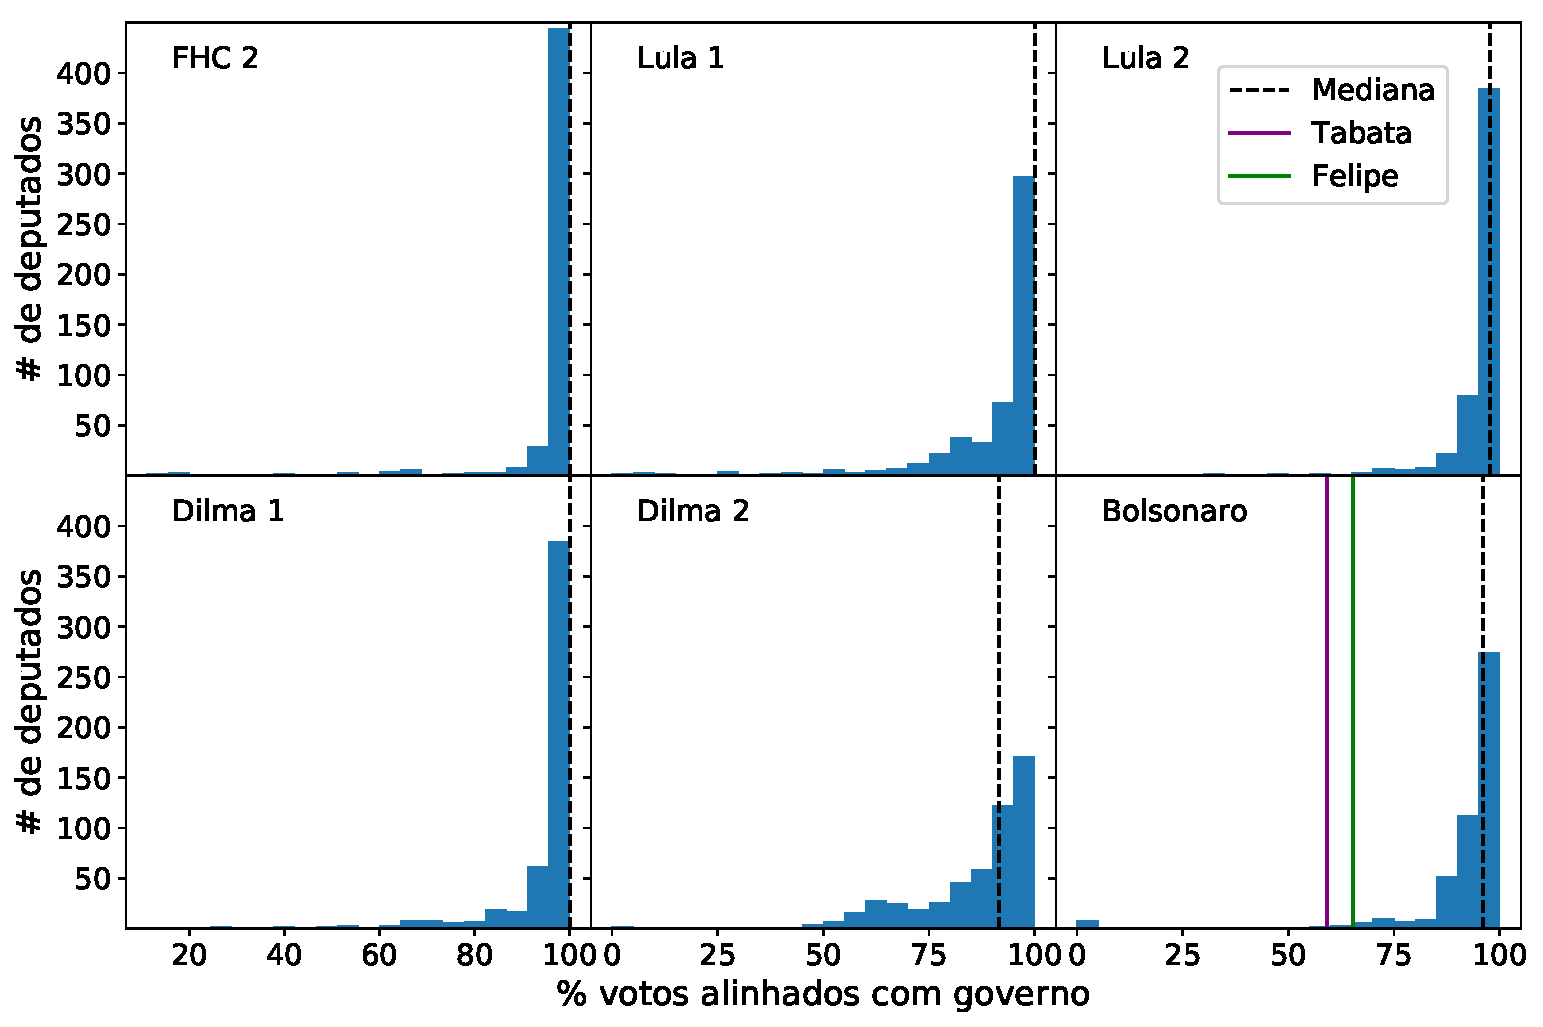
\includegraphics[width=1.0\textwidth]{graficos/apoio_ao_governo_deputados_2019-05-03.pdf}
\caption{Contagem do número de deputados em função da fração de seus votos no plenário que se
  alinham com a orientação do governo. Cada painel apresenta os dados dos 100 primeiros dias de
  cada legislatura, discriminadas pelo presidente no período. A linha vertical tracejada preta
  separa a metade dos deputados com maior e menor apoio e as linhas coloridas indicam a posição
  dos parlamentares do Acredito.}
\label{fig:apoio-governo-deputados}
\end{figure} 

Na maioria das legislaturas, a distribuição bimodal indica uma separação clara dos deputados
entre governo e oposição, sendo esta última contrária ao governo em mais de 2/3 das vezes.
Esse padrão se altera no primeiro mandato de Luiz Inácio Lula da Silva e no segundo mandato de Dilma.

A Fig. \ref{fig:apoio-governo-deputados} ainda indica que o governo de Jair Messias Bolsonaro detém
razoável apoio dos deputados, com distribuição similar à de governos anteriores. Esse dado contrasta
com a impressão derivada da cobertura da mídia, conforme mostra as manchetes da Fig. \ref{fig:manchetes-apoio}.
Uma hipótese para explicar essa aparente discrepância é que as manchetes em geral comentam sobre
a falta de articulação política no contexto da reforma da previdência, uma votação mais polêmica e
que exige um apoio maior (por se tratar de uma mudança na constituição). Outras hipóteses seriam
que a agenda de votações não está sendo comandada pelo governo ou que a orientação do governo esteja
seguindo os votos dos deputados ao invés de liderá-los.

\begin{figure}[H]
  \centering
  %\fbox{
    %\begin{minipage}{\textwidth}
      \fbox{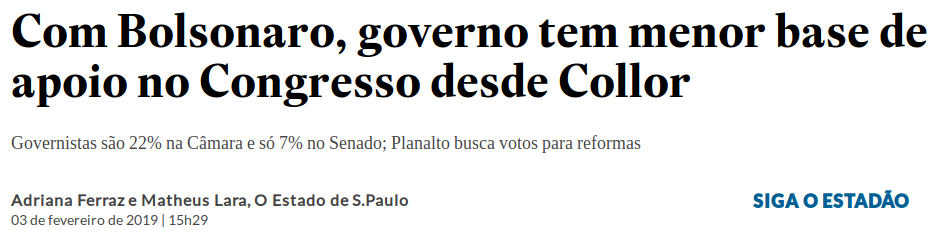
\includegraphics[width=1.0\textwidth]{manchetes/estadao-bolsonaro-menor-base.png}}
      \fbox{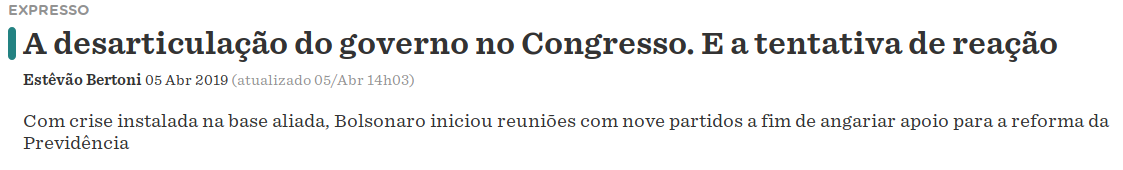
\includegraphics[width=1.0\textwidth]{manchetes/nexo-desarticulacao.png}}
      \fbox{
\includegraphics[width=1.0\textwidth]{manchetes/forum-PSL-ameaca-rebeliao.png}}
    %\end{minipage}
    %}
\caption[Exemplos de manchetes mencionando dificuldades do governo com o congresso, extraídas dos jornais
  O Estado de São Paulo e Nexo, e da Revista Fórum.]{Exemplos de manchetes mencionando dificuldades do governo com o congresso, extraídas dos jornais
  O Estado de São Paulo e Nexo, e da Revista Fórum.\footnotemark}
\label{fig:manchetes-apoio}
\end{figure}
\footnotetext{\\\tinyurl{http://politica.estadao.com.br/noticias/geral,com-bolsonaro-governo-tem-menor-base-de-apoio-no-congresso-desde-collor,70002706224}\\
  \tinyurl{http://www.nexojornal.com.br/expresso/2019/04/05/A-desarticula\%C3\%A7\%C3\%A3o-do-governo-no-Congresso.-E-a-tentativa-de-rea\%C3\%A7\%C3\%A3o}\\
  \tinyurl{https://www.revistaforum.com.br/parlamentares-do-psl-ameacam-rebeliao-contra-o-governo-jair-bolsonaro}}

Também analisamos o apoio ao governo por votação. A Fig. \ref{fig:apoio-governo-votacao} mostra o resultado
desse levantamento para os 100 primeiros dias das legislaturas desde 1999. Vemos que o segundo mandato
de Fernando Henrique obteve maioria absoluta (257 votos) em todas as votações dos 100 primeiros dias; já
o segundo mandato de Dilma é o único que não conseguiu que a média do número de votos por votação
superasse 257. Foi também nesse governo em que se registrou o maior número de votações em 100 dias.
O atual governo apresentou características típicas dos governos anteriores, com apoio médio
acima da maioria absoluta e um número mais baixo de votações.

\begin{figure}[H]
\centering
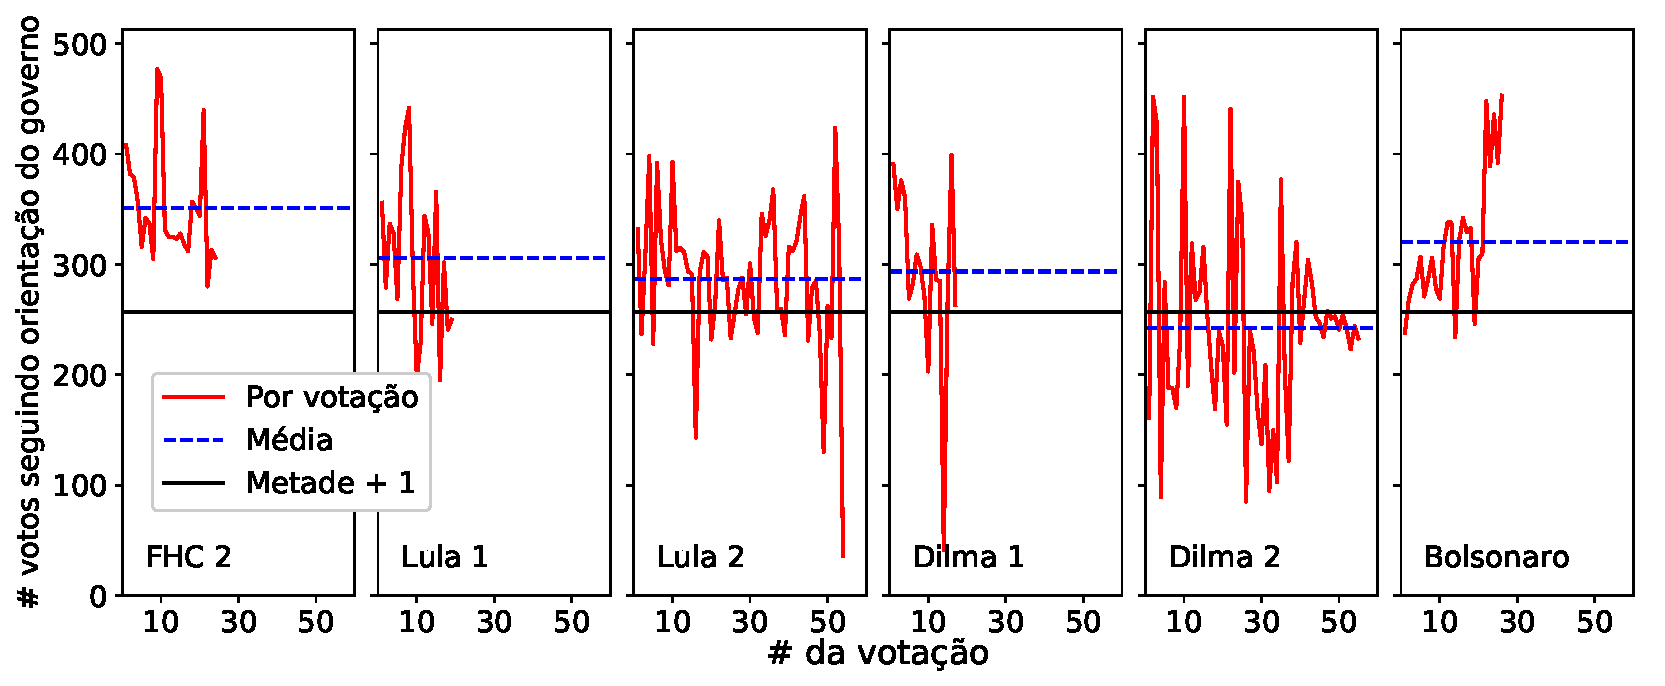
\includegraphics[width=1.0\textwidth]{graficos/apoio_ao_governo_por_votacao_2019-05-03.pdf}
\caption{Número de votos seguindo a orientação do governo, em cada votação dos 100 primeiros
  dias de congresso (em vermelho). Cada painel apresenta uma legislatura diferente, que teve
  um número diferente de votações nos 100 primeiros dias. A linha tracejada azul indica a média
  do número de votos obtidos em cada votação, e a linha contínua preta representa o mínimo de
  votos para se obter maioria absoluta (metade do total de deputados mais um).}
\label{fig:apoio-governo-votacao}
\end{figure} 

O alinhamento com o governo atual também foi estimado por partido. Nesse caso, os
partidos foram classificados de acordo com a sistematicidade com a qual seguiram
a orientação dos governos desde 1999. Aqueles que apresentaram uma taxa de apoio
superior a 80\% em todos os governos nos quais possuíam representantes na câmara
(com exceção do segundo mandato de Dilma, que perdeu apoio de maneira generalizada) foram
denomidados ``governativos''. Partidos sem presença nas legislaturas anteriores à $55^{\mathrm{\underline{a}}}$ (e.g. PROS),
foram classificados como ``indefinido''. 

A Fig. \ref{fig:apoio-governo-partido} mostra que o apoio ao governo atravessa múltiplos partidos e que,
dentre aqueles com mais de 80\% de votos, cerca de 40\% foram classificados como governativos. Nessa classificação
é importante ressalvar que alguns partidos tiveram sua composição e tamanho significativamente alterados ao longo
do tempo (e.g. PSL), de forma que seu comportamento no passado pode não ter relação com seu
comportamento atual. Do conjunto de partidos mais próximos ao governo, talvez seja mais interessante ressaltar aqueles
não classificados como governativos e que estiveram presentes em legislaturas anteriores: DEM, Cidadania (ex-PPS) e PSDB.

\begin{figure}[H]
\centering
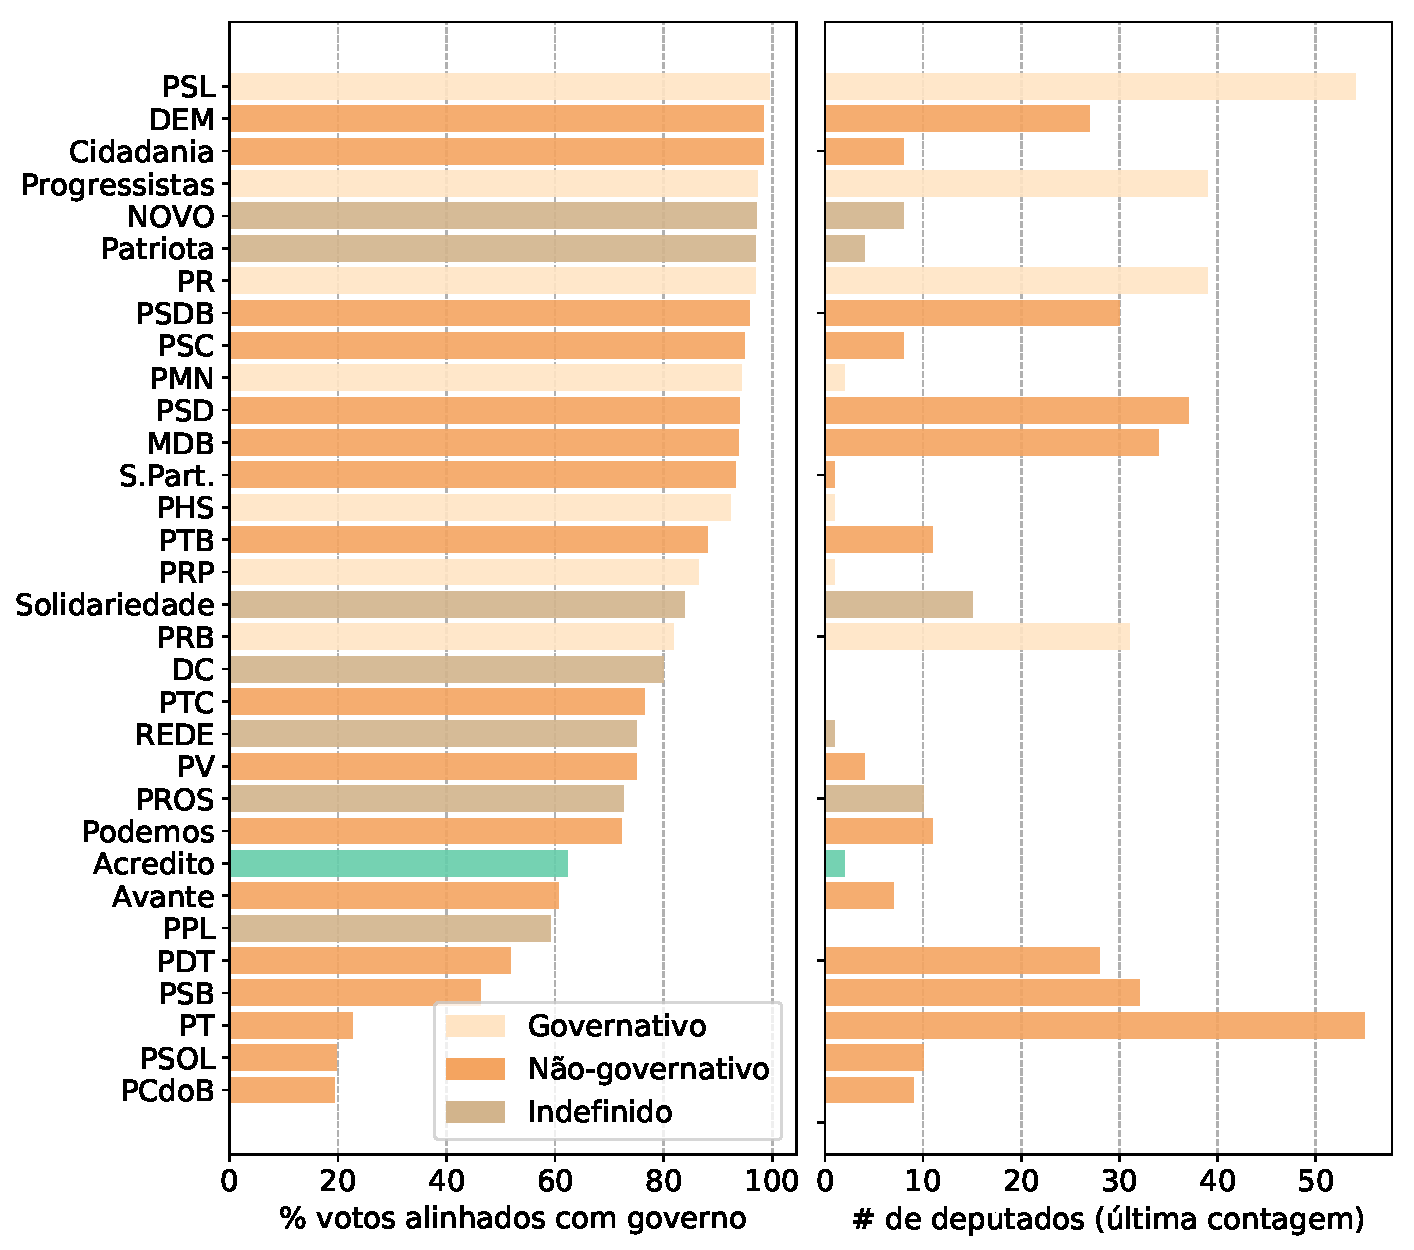
\includegraphics[width=1.0\textwidth]{graficos/apoio_ao_governo_partidos+tamanho_2019-05-03.pdf}
\caption{Fração de votos dos deputados que foram alinhados com a orientação do governo atual (painel esquerdo), e
  número de deputados de acordo com a última filiação, dentro de cada partido. O conjunto de votos dos dois
  parlamentares do Acredito aparece em verde.}
\label{fig:apoio-governo-partido}
\end{figure} 

Vemos na Fig. \ref{fig:apoio-governo-partido} que o grau de alinhamento com o governo varia de maneira
mais ou menos suave para a maioria dos partidos. Exceção a esse comportamento se dá com o PT, PSOL e
PCdoB, que formam uma oposição mais demarcada. A Fig. \ref{fig:apoio-governo-partido-G} apresenta os
mesmos dados mas apenas para os partidos com 20 deputados ou mais.

\begin{figure}[H]
\centering
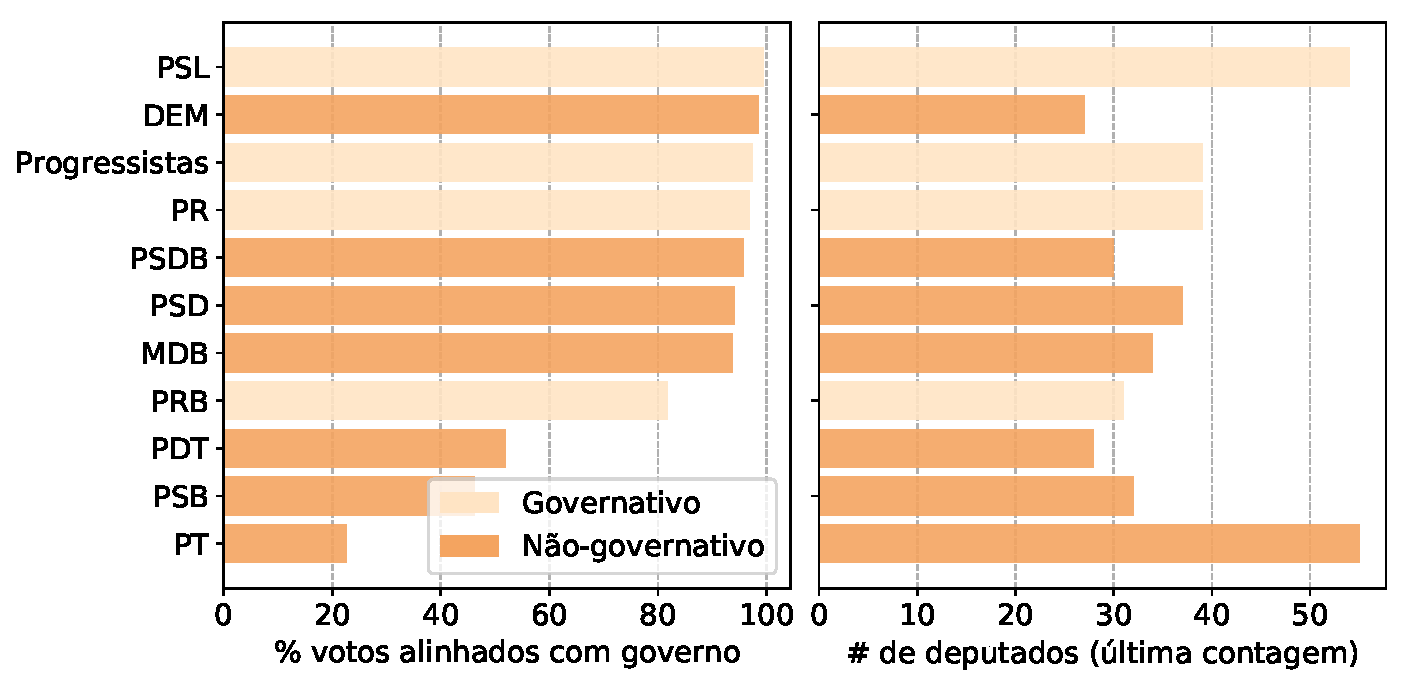
\includegraphics[width=1.0\textwidth]{graficos/apoio_ao_governo_partidosG+tamanho_2019-05-03.pdf}
\caption{Igual à Fig. \ref{fig:apoio-governo-partido}, mas para partidos com 20 deputados ou mais.}
\label{fig:apoio-governo-partido-G}
\end{figure} 

\subsubsection{Fidelidade partidária}

Para estimar a fidelidade partidária, verificamos a fração de votos dos deputados que seguem
a orientação do próprio partido. Novamente, votações nas quais não houve orientação foram
ignoradas. É importante ressaltar que alguns partidos orientaram poucas vezes e/ou são compostos
por poucos parlamentares, o que resulta em amostras pequenas e com pouca representatividade estatística.
A Tabela \ref{tab:alinha-dep} mostra o número de orientações recebidas por cada deputado.

A Fig. \ref{fig:fid-poder-partido} mostra que, tanto atual quanto historicamente, a maioria dos partidos
apresentam alta fidelidade, com mais de 80\% dos votos de seus deputados alinhados à sua orientação.
Para a maioria dos partidos, também observamos um ligeiro aumento do grau de fidelidade na legislatura atual.

\begin{figure}[H]
\centering
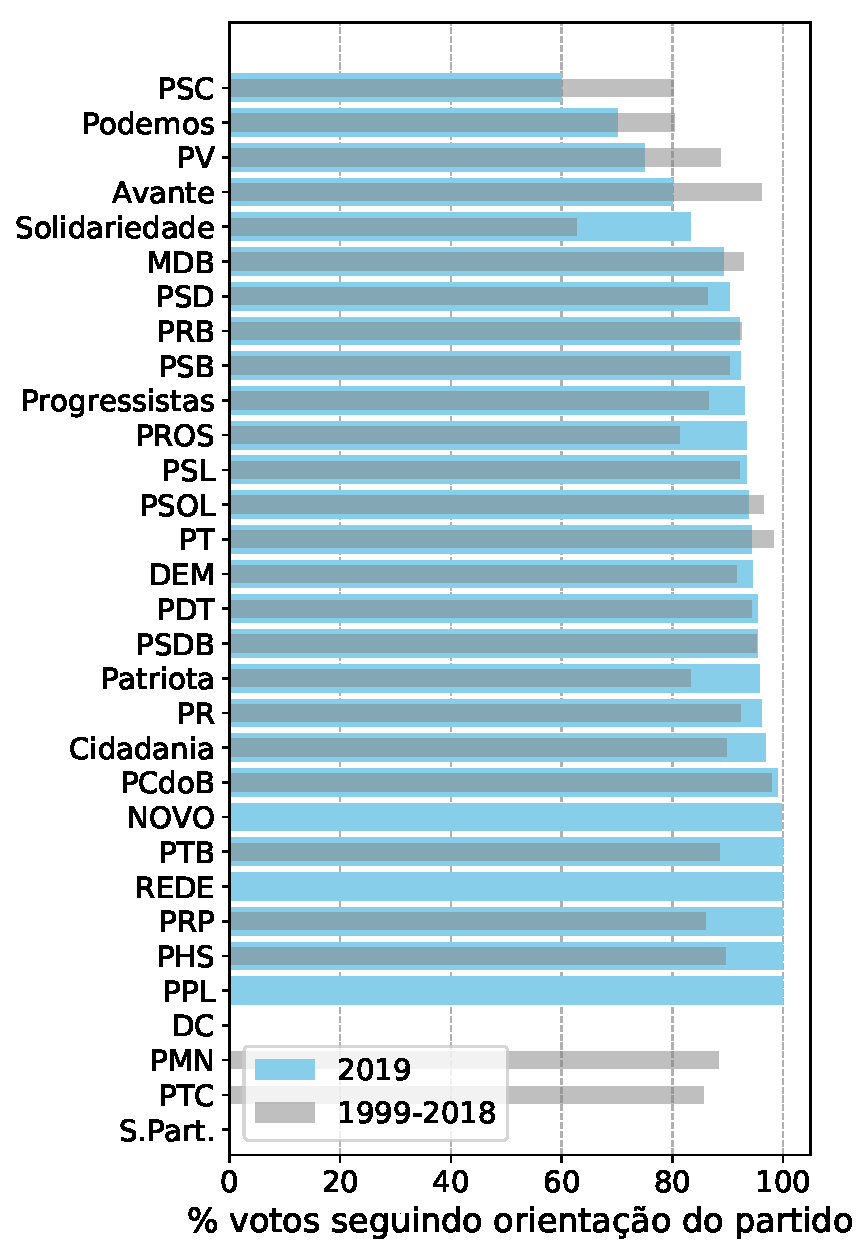
\includegraphics[width=0.49\textwidth]{graficos/fidelidade_partidaria_media_2019-05-03.pdf}
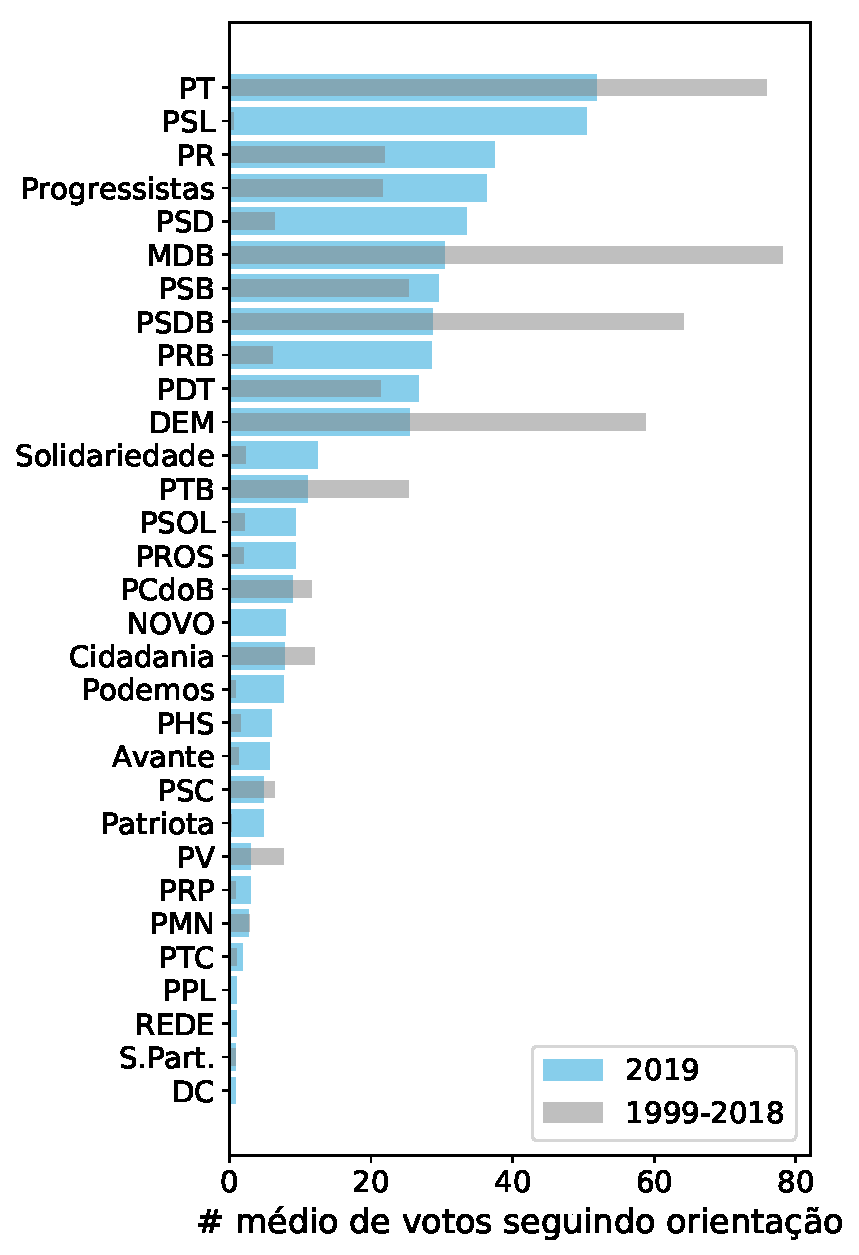
\includegraphics[width=0.49\textwidth]{graficos/poder_partidario_2019-05-03.pdf}
\caption{O painel esquerdo mostra a fração dos votos dos deputados que seguem orientação do próprio partido, e
  o painel direito mostra o número médio de votos que seguem a orientação do próprio partido.
  As barras azuis e largas são para a atual legislatura, e as cinzas e estreitas são para o período
  histórico de 2011 a 2019.
}
\label{fig:fid-poder-partido}
\end{figure} 

O painel direito dessa figura apresenta o grau de fidelidade (painel esquerdo) multiplicado pelo tamanho da bancada
(ou tamanho médio, no caso do período histórico), o que dá o número de votos que o partido consegue
obter dada uma certa orientação. Uma vez que a fidelidade partidária não varia muito entre os partidos,
aqueles com as maiores bancadas (e.g. PT e PSL em 2019, MDB na série histórica) são também os que podem
orientar a maior quantidade de votos. Aqui destacamos que partidos outrora numerosos na câmara perderam
muitos assentos na legislatura atual (PT, PSDB, MDB e DEM), enquanto outros partidos, como o PSL e PRB,
tiveram crescimento significativo. De maneira geral, observamos na atualidade uma distribuição das
cadeiras entre um número maior de partidos.

\begin{figure}[H]
\centering
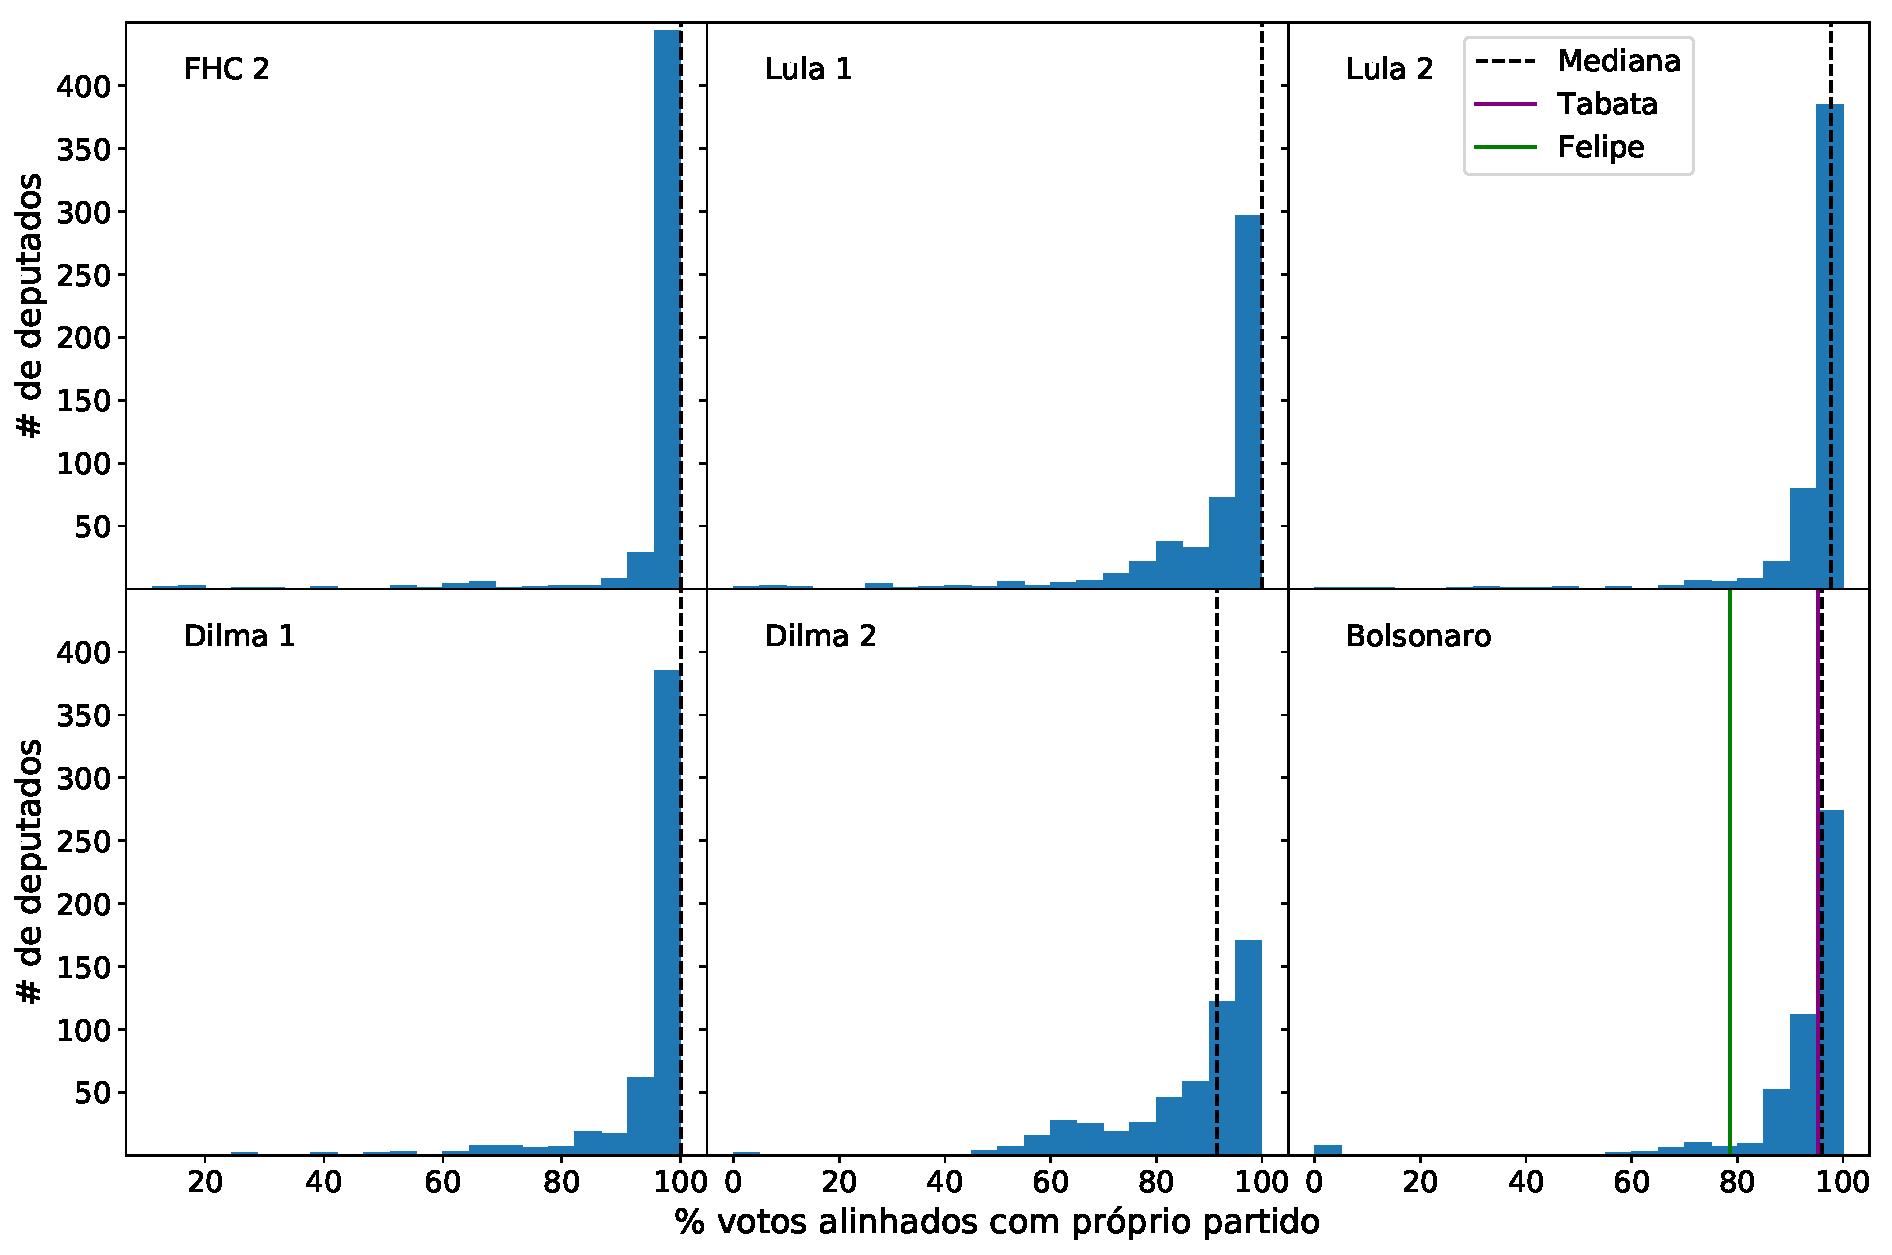
\includegraphics[width=1.0\textwidth]{graficos/fidelidade_partidaria_deputados_2019-05-03.pdf}
\caption{Histogramas da fração de votos dos deputados que são alinhados com o próprio partido, um para
  cada 100 primeiros dias de legislatura. A linha vertical preta indica a mediana e as linhas
  coloridas, o alinhamento dos parlamentares do Acredito com seus respectivos partidos.}
\label{fig:fid-poder-deputado}
\end{figure} 

Por fim, a Fig. \ref{fig:fid-poder-deputado} mostra a distribuição dos deputados de várias legislaturas
em termos de fidelidade partidária. De maneira geral, ela é altamente concentrada em altos valores. Vemos
que a situação atual não difere muito do comportamento histórico e que, nos 100 primeiros dias da legislatura
anterior (segundo mandato de Dilma), a fidelidade partidária apresentou uma queda. 


%%%%%%%%%%%%%%%%%%%%%%%%%%%%%%%%%%%%%%%%%%
\subsection{Distribuição de cargos e poder}

A proposta desta seção é verificar como os cargos em comissões e lideranças de blocos e partidos,
de maneira conjunta, são distribuídos entre os deputados. Aqui, infelizmente, temos dificuldades com a base de dados
abertos da câmara: parlamentares cuja participação em comissões é conhecida ou listada no portal
da câmara não aparecem como participantes dos órgãos. Os casos da deputada Tabata
Amaral\footnote{\footurl{http://www.camara.leg.br/deputados/204534}\\
  \footurl{https://dadosabertos.camara.leg.br/api/v2/deputados/204534/orgaos?ordem=ASC\&ordenarPor=dataInicio}}
(membro titular na Comissão de Educação) e do deputado
Ted Conti\footnote{\footurl{http://www.camara.leg.br/deputados/206231}\\
  \footurl{https://dadosabertos.camara.leg.br/api/v2/deputados/206231/orgaos?ordem=ASC\&ordenarPor=dataInicio}}
(membro titular na Comissão de Ciência e Tecnologia, Comunicação e Informática) são exemplos desse
problema. A Fig. \ref{fig:orgaos-por-ano} mostra que o ano de 2019 apresenta um registro atípico de número
de vagas preenchidas para um início de legislatura, evidenciando o problema. Além disso, e figura mostra que dados anteriores a 1999 estão
ausentes.

\begin{figure}[H]
\centering
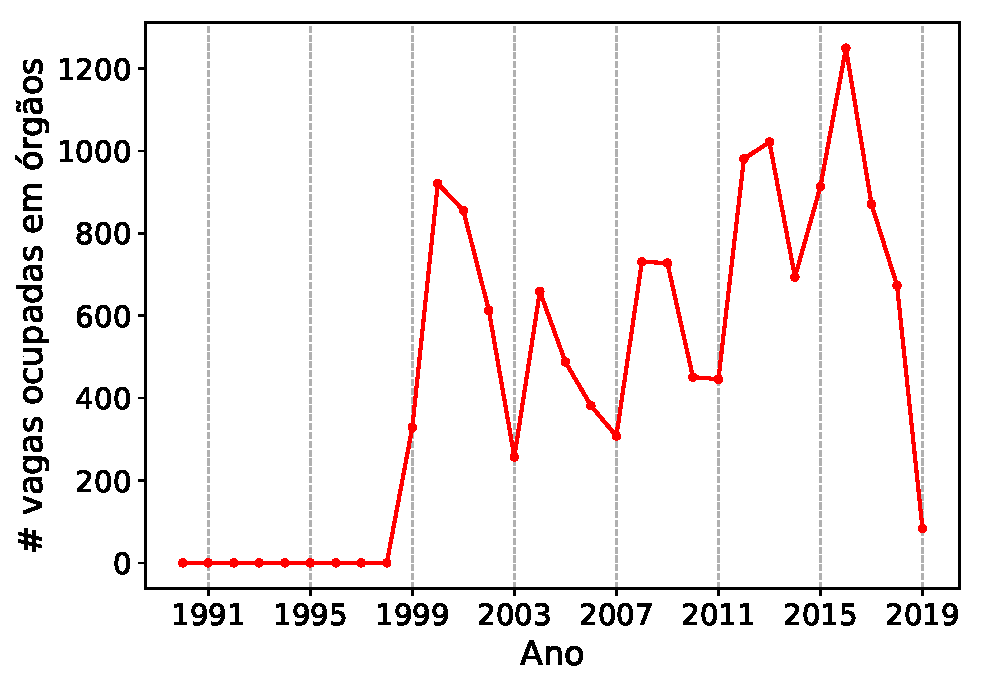
\includegraphics[width=0.7\textwidth]{graficos/orgaos-ocupados-por-ano_2019-05-02.pdf}
\caption{Número de vagas preenchidas por deputados no período de 1 de fevereiro a 18 de abril em órgãos (incluindo Mesa Diretora,
  Grupos de Trabalho, Comissões Parlamentares de Inquérito, Comissões Permanentes, Especiais, Mistas e Externas,
  Conselhos e Subcomissões, entre outros) ao longo dos anos, de acordo com a base de dados abertos da câmara dos deputados.}
\label{fig:orgaos-por-ano}
\end{figure} 

Pelo motivo apresentado acima, apenas uma análise histórica da participação em comissões pode ser feita. Por outro lado,
a base de dados abertos não guarda as informações sobre lideranças passadas dos blocos e partidos, de maneira
que não é possível realizar uma análise histórica conjunta entre participação em comissões e lideranças.

\HX{Incluir análise histórica da distribuição de cargos}

%%%%%%%%%%%%%%%%%%%%%%%%%%%%%%%%%%%
\subsection{Atividade parlamentar}

\HX{Incluir seção sobre atividade parlamentar na câmara e no senado}

%%%%%%%%%%%%%%%%%%%%%%%%%%%%%%%%%%%
\subsection{Uso da cota parlamentar}

Conforme apresentado na Seção \ref{sec:intro}, as bases de dados relacionadas às despesas parlamentares dos 100 últimos
dias ainda estão sendo atualizadas. As referentes ao ano de 2018 ganharam, em média, 530 entradas por dia desde o início
dessa análise, em grande parte relativas à emissão de bilhetes aéreos. Essa incompleteza da base de dados se evidencia
na Fig. \ref{fig:n-despesas-por-mes}. A queda abrupta, a partir de 2018, no número de despesas registradas é ao menos
em parte consequência dessa defasagem no registro dos gastos. A Fig. \ref{fig:n-despesas-por-mes} ainda mostra que
os gastos do total de deputados segue um padrão recorrente ao longo dos anos, com uma queda significativa em janeiro.

\begin{figure}[H]
\centering
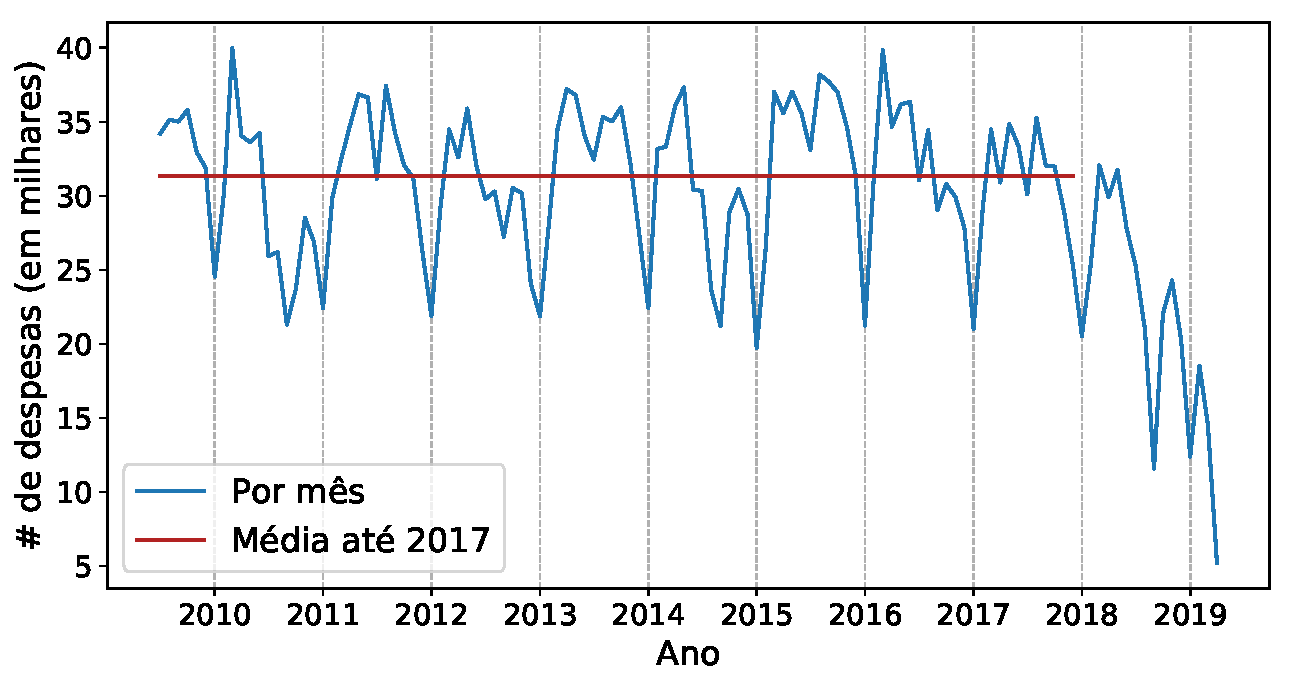
\includegraphics[width=1.0\textwidth]{graficos/n_despesas_por_mes_2019-04-29.pdf}
\caption{Número de despesas na base de dados de uso da cota parlamentar dos deputados federais
  referentes a cada mês, em função do tempo (em azul).
  A linha vermelha indica o número médio de 2009 a 2018.}
\label{fig:n-despesas-por-mes}
\end{figure} 

Para acompanhar o valor total gasto com a cota parlamentar ao longo do tempo, nós primeiro deflacionamos os
valores pelo IPCA e em seguida o decompusemos num modelo aditivo com termos de tendência geral, sazonalidade e
resíduo (veja a Fig. \ref{fig:total-despesas-por-mes}). Através da curva de tendência, podemos notar que
o valor médio gasto praticamente não se alterou desde 2010, sendo que uma leve queda pode ser notada em anos
recentes. Ressaltamos que ao menos parte dessa queda é consequência da defasagem de registro dos gastos.

\begin{figure}[H]
\centering
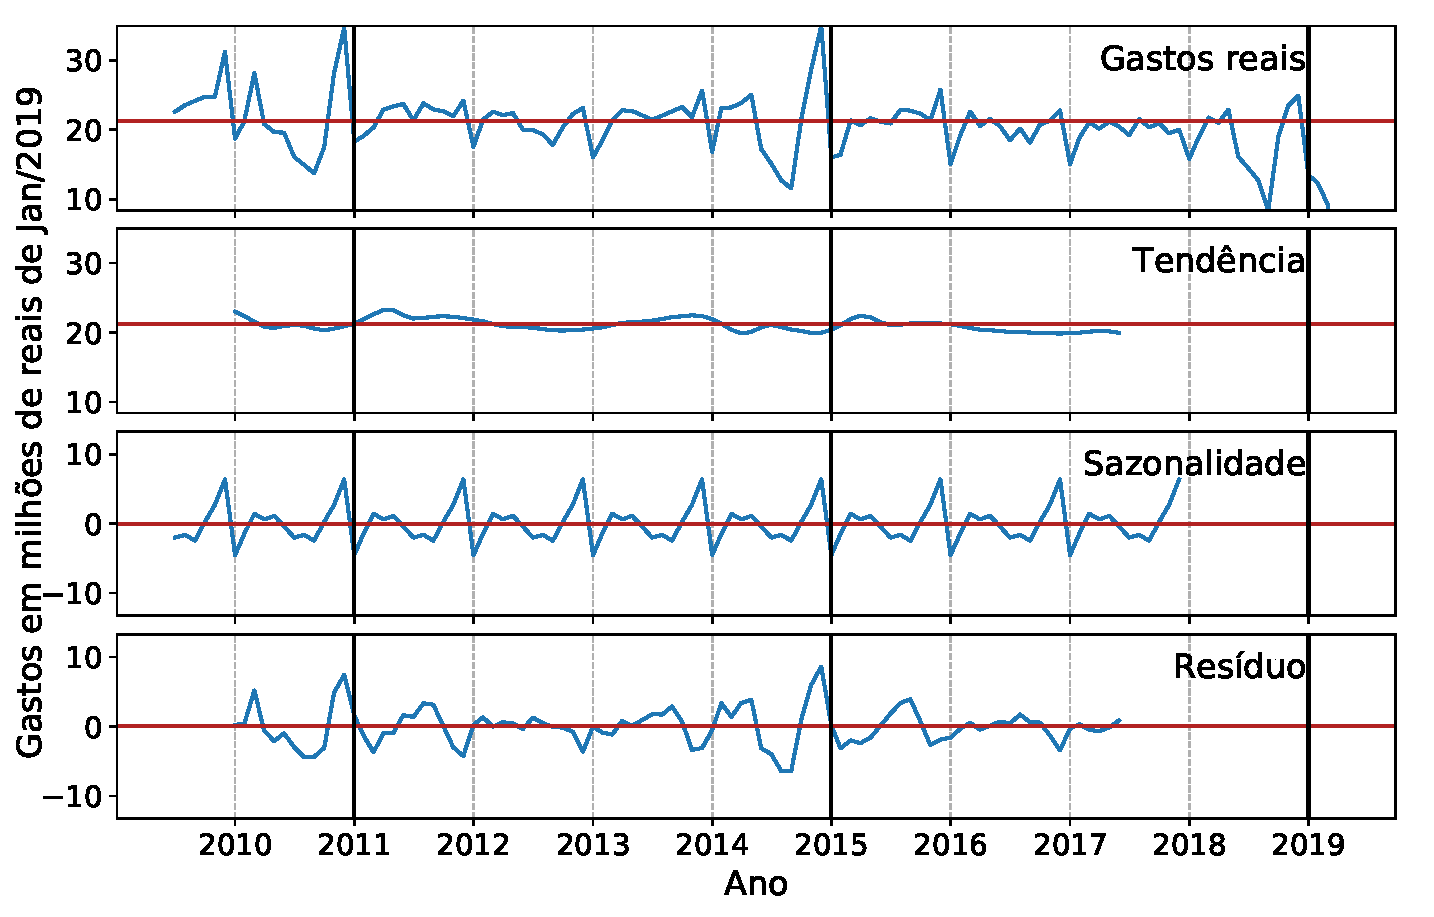
\includegraphics[width=1.0\textwidth]{graficos/despesas-reais-e-sazonalidade_2019-04-29.pdf}
\caption{Valor real (descontada a inflação) gasto com o exercício da atividade parlamentar em cada mês
  (reembolsos feitos dentro da cota parlamentar, em azul). O painel superior mostra o valor observado, e os
  abaixo mostram as contribuições de: tendência geral, calculada através de uma média móvel; sazonalidade; e resíduo.
  A linha vermelha indica o valor médio em todo o período (nos dois painéis superiores) e o zero (nos dois
  painéis inferiores). A decomposição em contribuições aditivas foi feita até o ano de 2017.}
\label{fig:total-despesas-por-mes}
\end{figure} 

Também é possível notar que os gastos apresentam uma sazonalidade bastante marcada, com quedas mais
acentuadas em janeiro e picos em dezembro. Esses picos podem decorrer do fato de que a cota parlamentar, mensal,
pode ser acumulada ao longo do ano mas não pode ser transferida para o exercício financeiro seguinte.
É possível percebem ainda, tanto nos gráficos do valor observado quanto no de resíduos, que existe
um pico ainda mais acentuado ao final de cada legislatura (marcadas com linhas verticais pretas contínuas).
Esse pico parece ser precedido por uma queda nos gastos, possivelmente indicando uma estratégia de acúmulo de verba
para a realização de um último gasto em dezembro.

Por fim, verificamos como o valor total reembolsado pela cota parlamentar se divide nas categorias pré-definidas
pela câmara. A Figura \ref{fig:despesas-por-tipo} mostra a fração do valor total que é destinada a cada categoria
de gastos. Verificamos que os maiores gastos realizados são com divulgação da atividade parlamentar (que, em geral,
apresentam valores altos para uma única despesa e perfazem 20\% do total) e com transporte aéreo: somando as rubricas
``emissão de bilhere aéreo'', ``locação ou fretamento de aeronaves'' e ``passagens aéreas'', temos cerca de
23\% dos gastos. Em grande medida, esse montante deriva do deslocamento semanal do deputado ao seu estado de origem.
Gastos com manutenção de escritório de apoio em seu estado, consultorias, telefonia e transportes terrestres vêm
em seguida. Junto com passagens aéreas, o transporte totaliza cerca de 44\% do total. Gastos com alimentação e
hospedagem fora do distrito federal totalizam, em média, menos de 2\% dos gastos.

\begin{figure}[H]
\centering
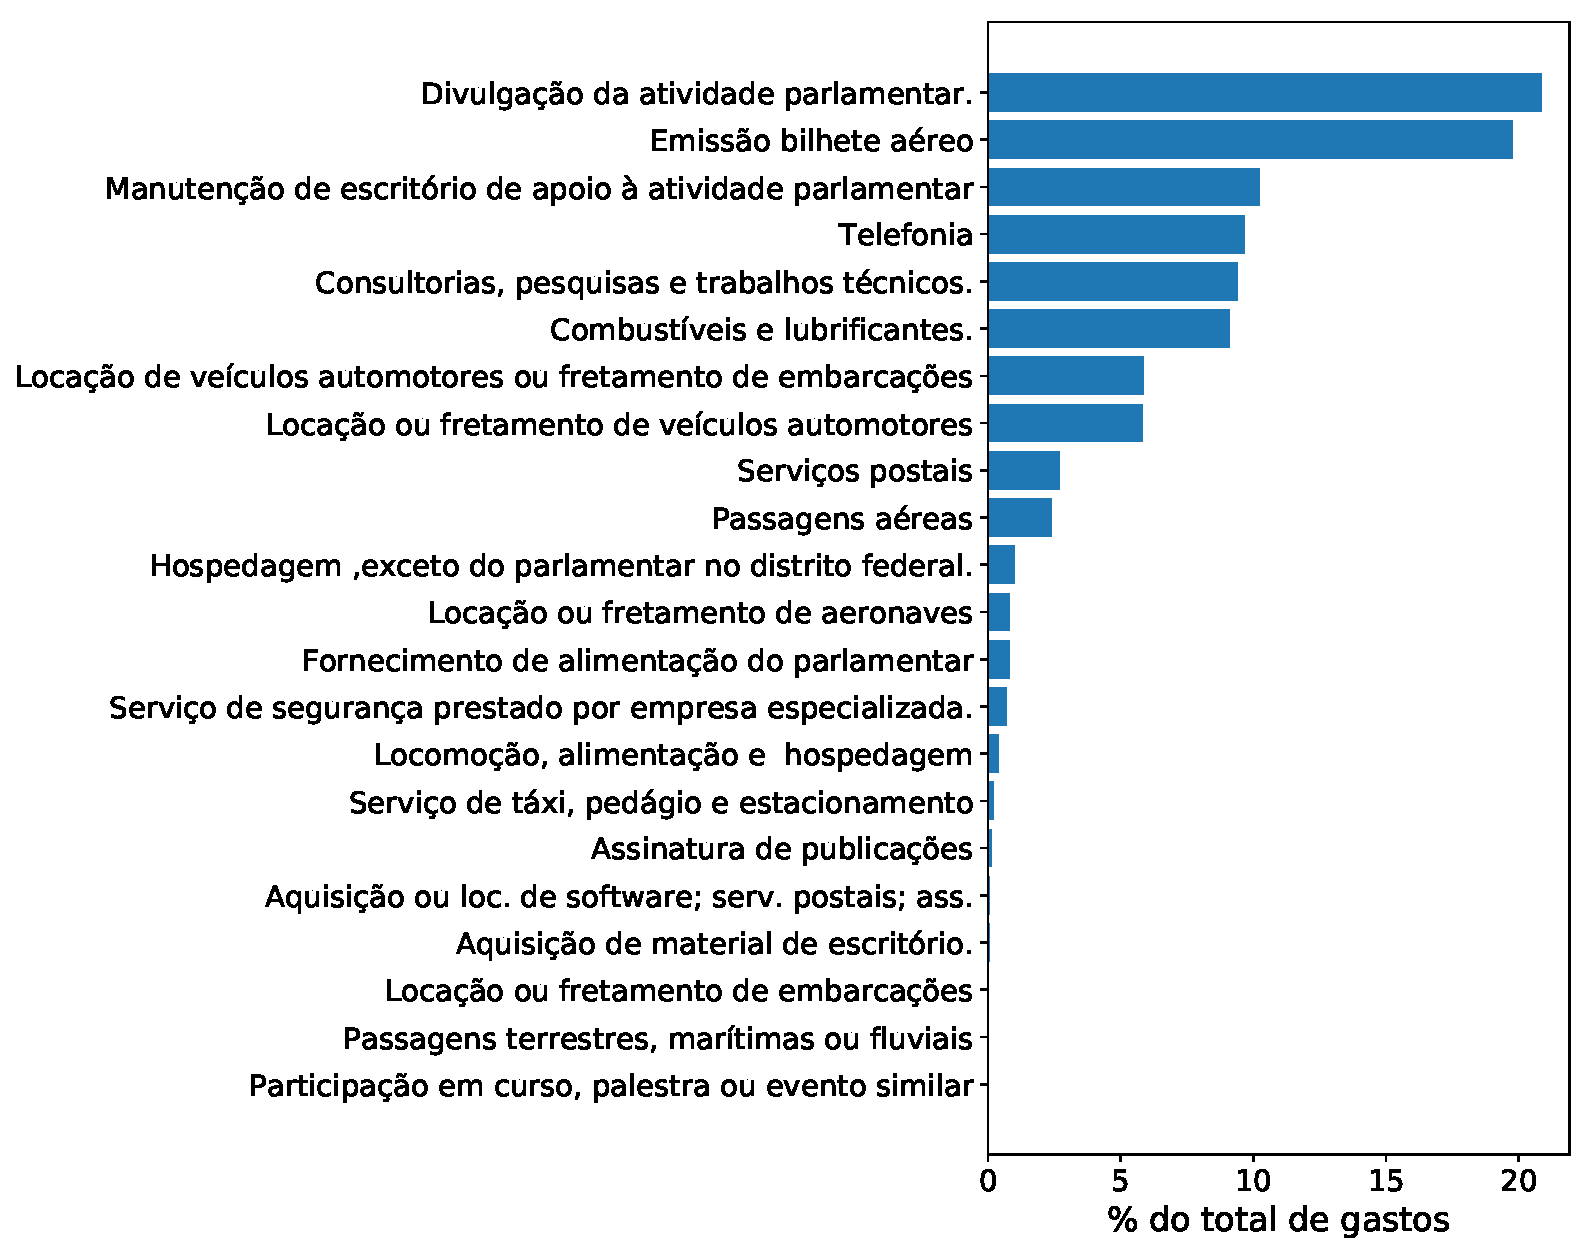
\includegraphics[width=1.0\textwidth]{graficos/total-despesas-por-tipo_2019-04-29.pdf}
\caption{Porcentagem do valor total utilizado pelos deputados federais que é destinado a cada finalidade. Nesse
cálculo, utilizamos os valores de 2009 a 2017, corrigigos pela inflação.}
\label{fig:despesas-por-tipo}
\end{figure} 



%%%%%%%%%%%%%%%%%%%%%%%%%%
\section{Proposições}

\subsection{Câmara dos deputados}

A base de dados abertos da câmara federal indica que, nos 100 primeiros dias da atual legislatura,
foram apresentados pouco mais de 1600 projetos de lei (PLs, veja a Fig. \ref{fig:prop-2019-tipo}),
o que resulta em, aproximadamente, 3,2 projetos por deputado. Dado que os PLs são a ampla maioria
das proposições apresentadas na legislatura atual, vamos focar nossa análise nesse tipo de proposição e
compará-las com os anos anteriores.

\begin{figure}[H]
\centering
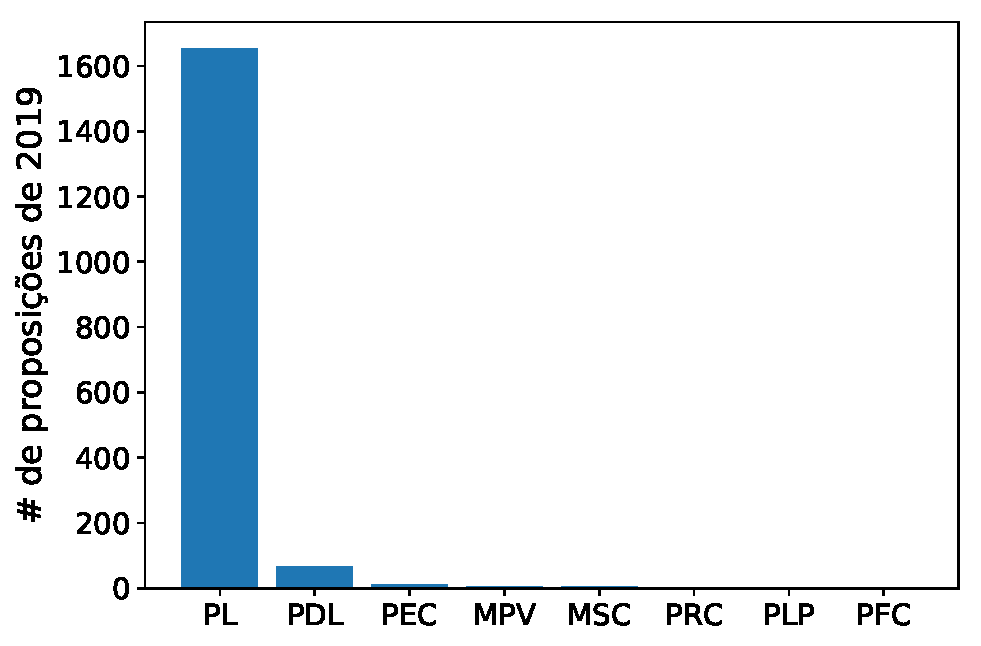
\includegraphics[width=0.7\textwidth]{graficos/proposicoes-2019-por-tipo_2019-05-01.pdf}
\caption{Número de proposições apresentadas na $56^{\mathrm{\underline{a}}}$ (atual) legislatura,
  classificadas por tipo: Projeto de Lei (PL), Projeto de Decreto Legislativo (PDL),
  Proposta de Emenda à Constituição (PEC), Medida Provisória (MPV), Mensagem de Acordos,
  convênios, tratados e atos internacionais (MSC), Projeto de Resolução da Câmara dos Deputados (PRC),
  Projeto de Lei Complementar (PLP) e Proposta de Fiscalização e Controle (PFC).}
\label{fig:prop-2019-tipo}
\end{figure} 

A Fig. \ref{fig:prop-por-ano} mostra a evolução do número de PLs apresentados ao longo do tempo,
tomando como referência o mesmo período a cada ano. Além do crescimento observado, é interessante
notar que os inícios de legislatura apresentam picos de apresentação de PLs.

\begin{figure}[H]
  \centering
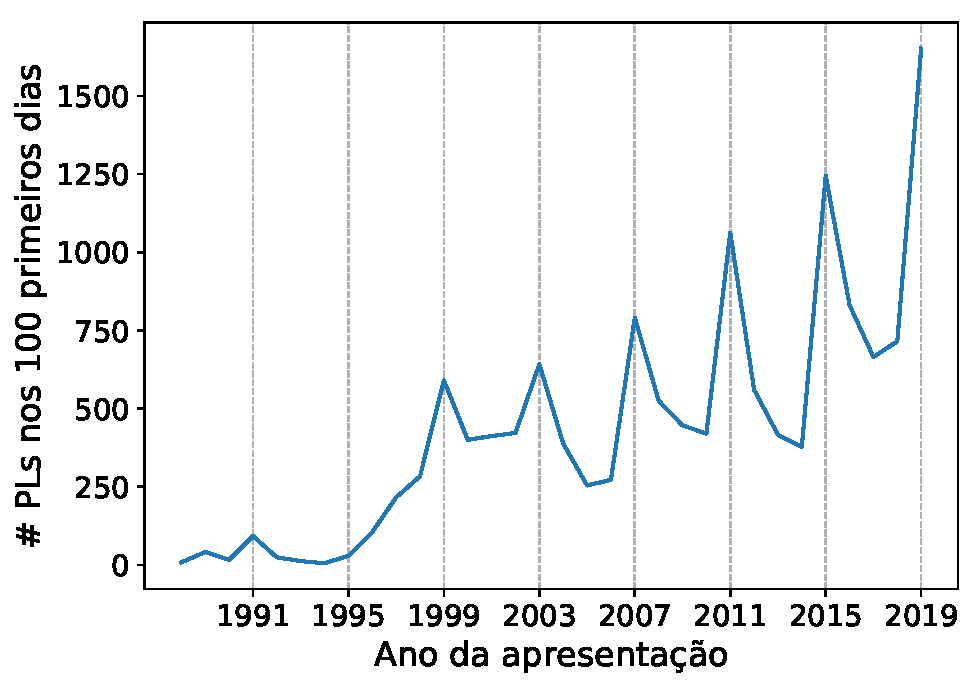
\includegraphics[width=0.7\textwidth]{graficos/PLs-por-ano_2019-05-03.pdf}
\caption{Evolução do número de PLs apresentados nos 100 dias a partir de 1 de fevereiro, de cada ano.
Os inícios de legislatura são marcados pelas linhas tracejadas cinzas.}
\label{fig:prop-por-ano}
\end{figure}

O Centro de Documentação e Informação da Câmara fornece uma classificação oficial em temas para as
proposições.\footnote{Conforme descrito em \footurl{https://dadosabertos.camara.leg.br/swagger/api.html}}
Nós verificamos a frequência com que cada tema apareceu em cada ano, de maneira que podemos saber
quais são os temas historicamente mais recorrentes nos projetos de lei e quais os temas mais em voga
na legislatura atual. A Fig. \ref{fig:pl-por-tema-camara} sintetiza os resultados, na qual comparamos
a frequência de cada tema nos projetos de lei apresentados nos 100 primeiros dias da atual legislatura com as médias das frequências
em todo o período de janeiro de 2011 a dezembro de
2018.\footnote{Uma versão simplificada desse gráfico é apresentada na Fig. \ref{fig:pl-por-tema-camara-simples}.}

A escolha desse período como referência
visa reduzir flutuações estatísticas (em comparação com intervalos menores de tempo) e evitar mudanças 
de comportamento abruptas e não plenamente entendidas que parecem ter ocorrido na passagem de 2010 a 2011
(conforme apresentamos abaixo). Além disso, verificamos não existir uma sazonalidade significativa
que justifique restringir o cálculo da média histórica aos 100 primeiros dias das legislaturas anteriores.

\begin{figure}[H]
\centering
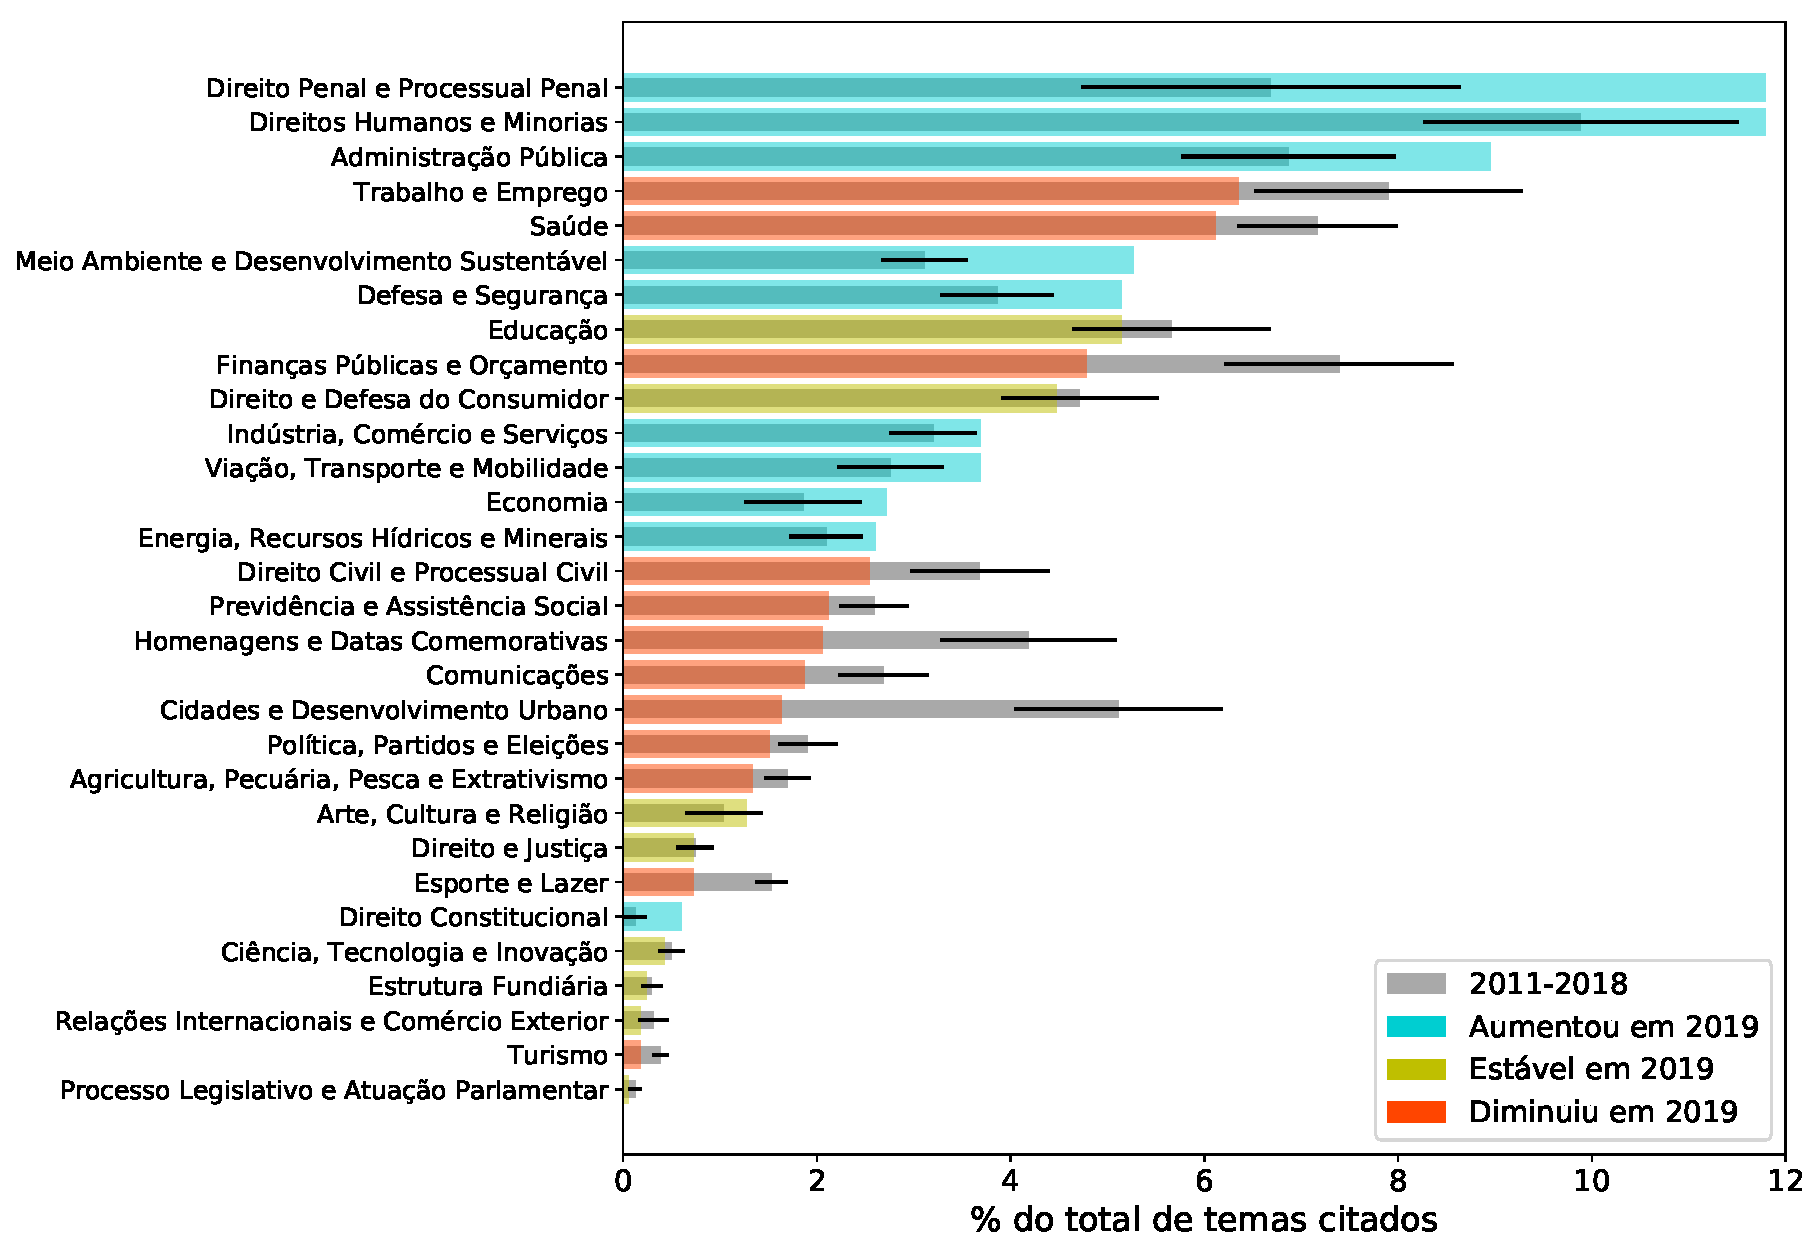
\includegraphics[width=1.0\textwidth]{graficos/temas_PL_fracao2019-vs-mediaAnterior_2019-05-03.pdf}
\caption{Frequência de cada tema (fração dos PLs apresentados que foram classificados naquele tema) na câmara.
  As barras cinzas e mais estreitas representam a média da frequência no período de janeiro de 2011 a
  dezembro de 2018, e as linhas pretas indicam a variação típica (desvio padrão) da frequência no período.
  As barras coloridas representam a frequência de cada tema para os 100 dias da atual legislatura.
  Frequências que cresceram mais que a variação típica dos anos anteriores estão em azul, e as que
  diminuíram mais que a variação típica estão em vermelho. As demais são apresentadas em amarelo.
  Os temas foram ordenados pela frequência atual.}
\label{fig:pl-por-tema-camara}
\end{figure}

Podemos notar que certos temas são, historicamente, mais frequentes que outros. No período desde 2011,
os três temas mais recorrentes foram de direitos humanos e minorias (10\%), trabalho e emprego (8\%)
e finanças públicas (7\%). Processo legislativo e atuação parlamentar, por outro lado, é tema de 0,1\%
dos PLs. Já na legislatura atual, os três temas mais comuns foram: direito penal e processual penal (12\%),
direitos humanos e minorias (12\%) e administração pública (9\%). Embora também fossem comuns nos anos
anteriores, esses temas sofreram alta, com destaque para a de direito penal e processual penal.

Os três temas que sofreram altas mais significativas foram: meio ambiente e desenvolvimento
sustentável (4,8$\sigma$, onde $\sigma$ é o desvio padrão da frequência de 2011 a 2018),
direito constitucional (4,2$\sigma$) e direito processual e penal (2,6$\sigma$). Os três
temas com baixas mais significativas foram: esporte e lazer (-4,9$\sigma$), cidades e desenvolvimento
urbano (-3,23$\sigma$) e turismo (-2,3$\sigma$). Hipotetizamos que as altas significativas
na fração de PLs apresentados indicam que os deputados estão buscando mudar as regras de jogo dentro
daquele tema em particular ou que aquele tema é prioridade para a membros da legislatura atual.
Baixas significativas podem indicar que as regras de jogo para aquele
tema são consideradas adequadas ou que o tema em questão não é prioridade para os deputados.

Conforme mencionado anteriormente, o ano de 2011 (que é um ano de início de legislatura)
marca uma mudança abrupta de comportamento para alguns temas. A Fig. \ref{fig:pl-agricultura}
exemplifica esse cenário: o tema ``estrutura fundiária'' passa de uma frequência de 2\% para outra
próxima de zero; já o tema ``Agricultura, Pecuária, Pesca e Extrativismo'' faz o caminho contrário.
Outros temas realizam transições semelhantes: direito e defesa do consumidor, direito e justiça, e
política, partidos e eleições também pulam de patamar em 2011; enquanto que viação, transporte e
mobilidade cai. Esses saltos podem indicar uma mudança na metodologia de classificação dos PLs.

\begin{figure}[H]
\centering
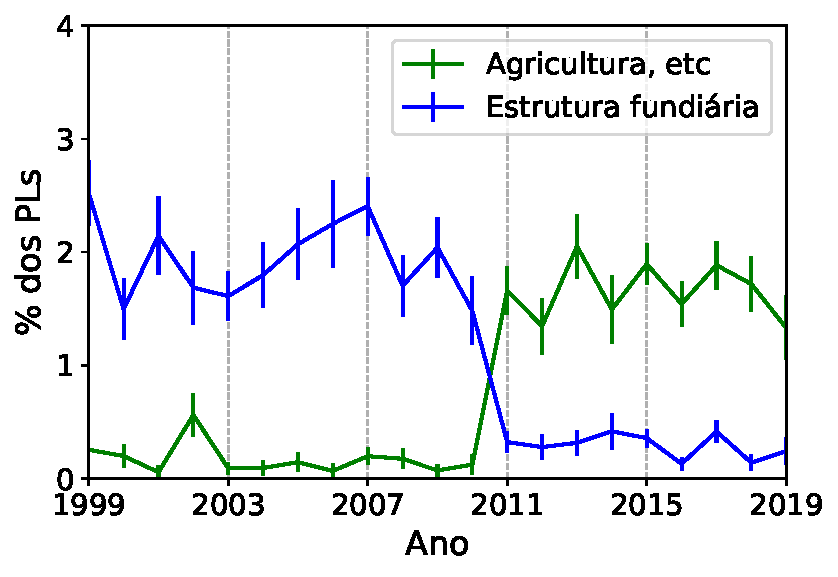
\includegraphics[width=0.6\textwidth]{graficos/PL-agricultura-por-ano_2019-05-01.pdf}
\caption{Evolução da frequência de PLs que tratam dos temas ``Agricultura, Pecuária, Pesca e Extrativismo''
  (em verde) e ``Estrutura fundiária'' (em azul), de 1999 a 2019. As barras de erro foram estimadas
assumindo que as contagems de PLs (dentro de um dado tema e de maneira agregada) sofrem flutuações de Poisson.}
\label{fig:pl-agricultura}
\end{figure}

Por fim, um achado interessante é a evolução da frequência do tema ``direitos humanos e minorias'' que,
no período analisado (de 1999 a 2019), passou por um crescimento significativo e substancial.
A Fig. \ref{fig:pl-direitos-humanos} mostra que, em 20 anos, esse tema dobrou de frequência, passando de
5\% para cerca de 11\%.

\begin{figure}[H]
\centering
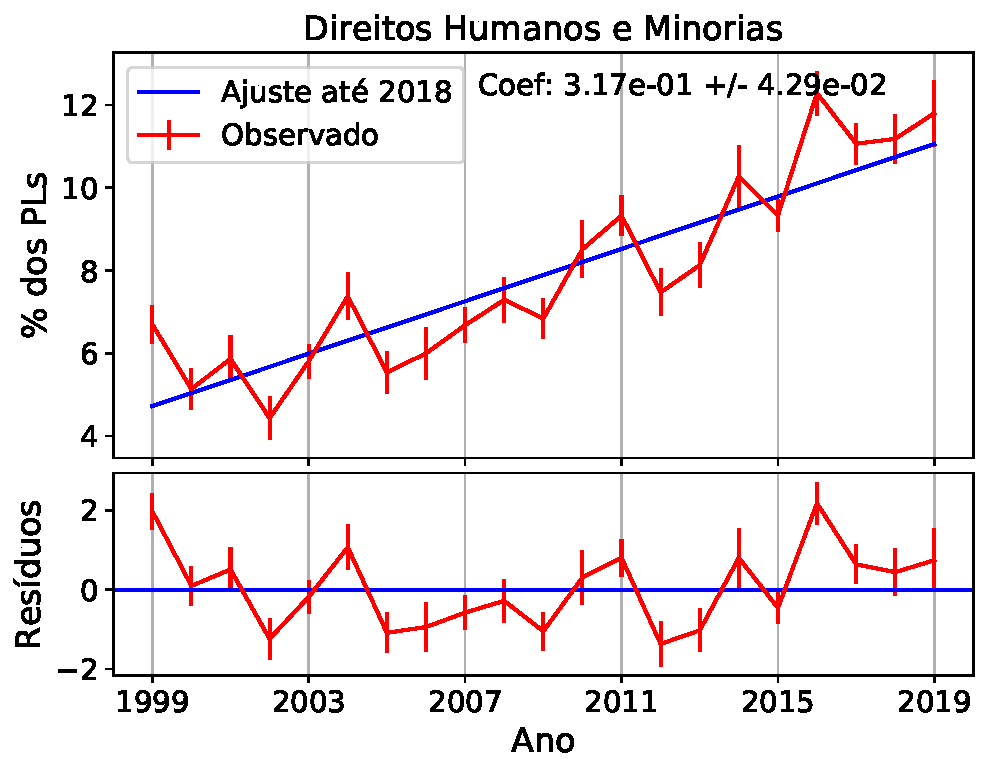
\includegraphics[width=0.7\textwidth]{graficos/PL-direitos-humanos-por-ano_2019-05-01.pdf}
\caption{O painel superior apresenta a evolução da frequência do tema ``direitos humanos e minorias''
  dentre os PLs apresentados; a linha vermelha mostra os valores observados, enquanto que a linha
  azul indica um ajuste linear com coeficiente angular $0,317\pm 0,043$. O painel inferior apresenta
  a diferença entre os valores observados e ajustados. As barras de erro foram estimadas assumindo
  flutuações de Poisson nas contagens de PLs.}
\label{fig:pl-direitos-humanos}
\end{figure}

\subsection{Senado}

A base de dados abertos do senado também classifica as proposições por temas, apesar dos temas serem
ligeiramente diferentes. A Fig. \ref{fig:pl-por-tema-senado} é análoga à Fig. \ref{fig:pl-por-tema-camara}, mas trata dos PLs apresentados
no senado.\footnote{Uma versão simplificada desse gráfico é apresentada na Fig. \ref{fig:pl-por-tema-senado-simples}.}

\begin{figure}[H]
\centering
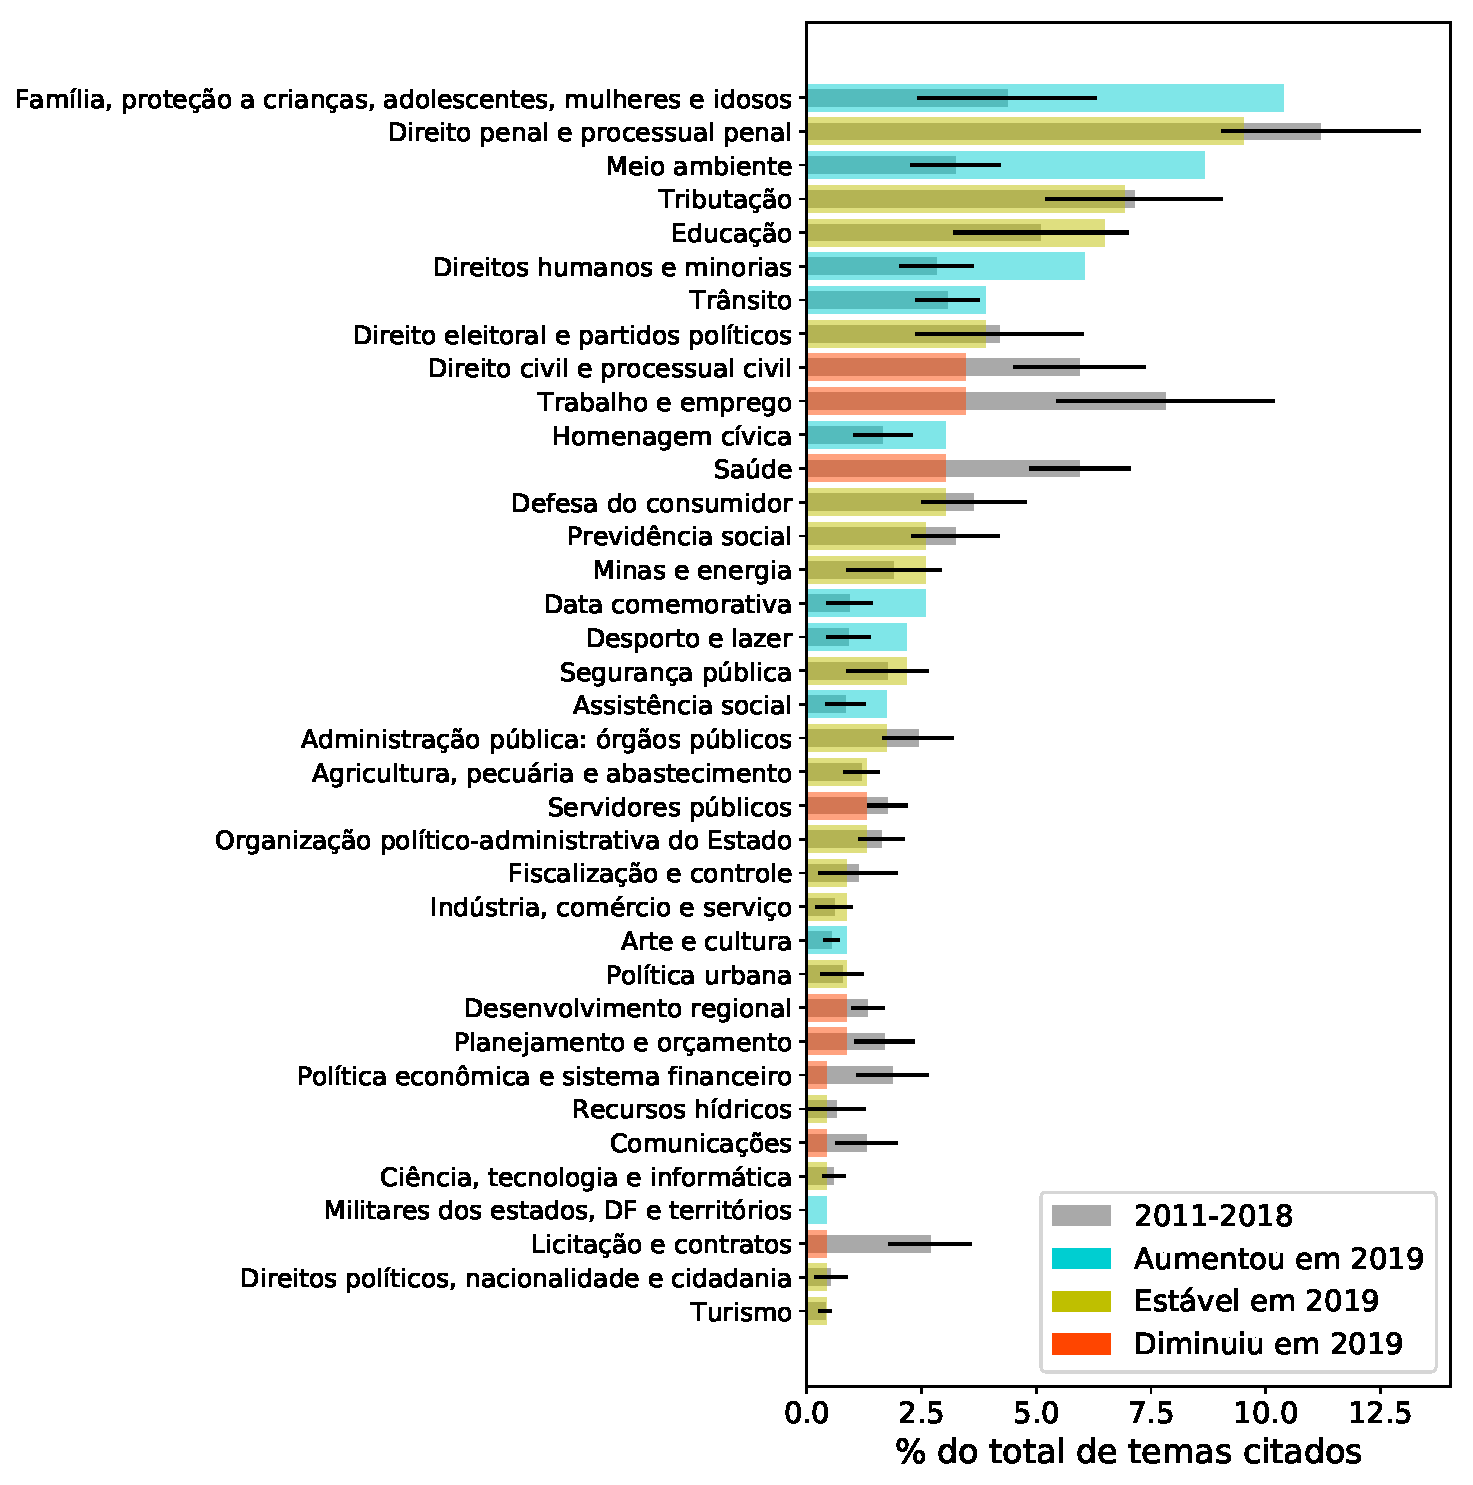
\includegraphics[width=1.0\textwidth]{graficos/senado/pls-temas-senado-r-completo.pdf}
\caption{Frequência de cada tema (fração dos PLs apresentados que foram classificados
  naquele tema) no senado. A representação e a forma de calcular a média histórica são iguais
  aos da Fig. \ref{fig:pl-por-tema-camara}.}
\label{fig:pl-por-tema-senado}
\end{figure}

Aqui, vemos algumas semelhanças à configuração de temas da câmara: os temas mais comuns são
próximos (direito penal e processual penal, direitos humanos e minorias e meio ambiente), e
também contrastam com temas como turismo e ciência e tecnologia (com baixa frequência).
As altas em 2019 dos temas ``meio ambiente'' e ``direitos humanos e minorias'' também aparecem,
enquanto que a de ``direito penal e processual penal'', não. Também notamos a repetição dos
padrões de queda nos temas ``trabalho e emprego'' e ``saúde''.
A base de dados abertos do senado também classifica as proposições em macro-temas, e suas frequências
históricas e em 2019 são apresentadas na Fig. \ref{fig:pl-por-macrotema-senado}.

\begin{figure}[H]
\centering
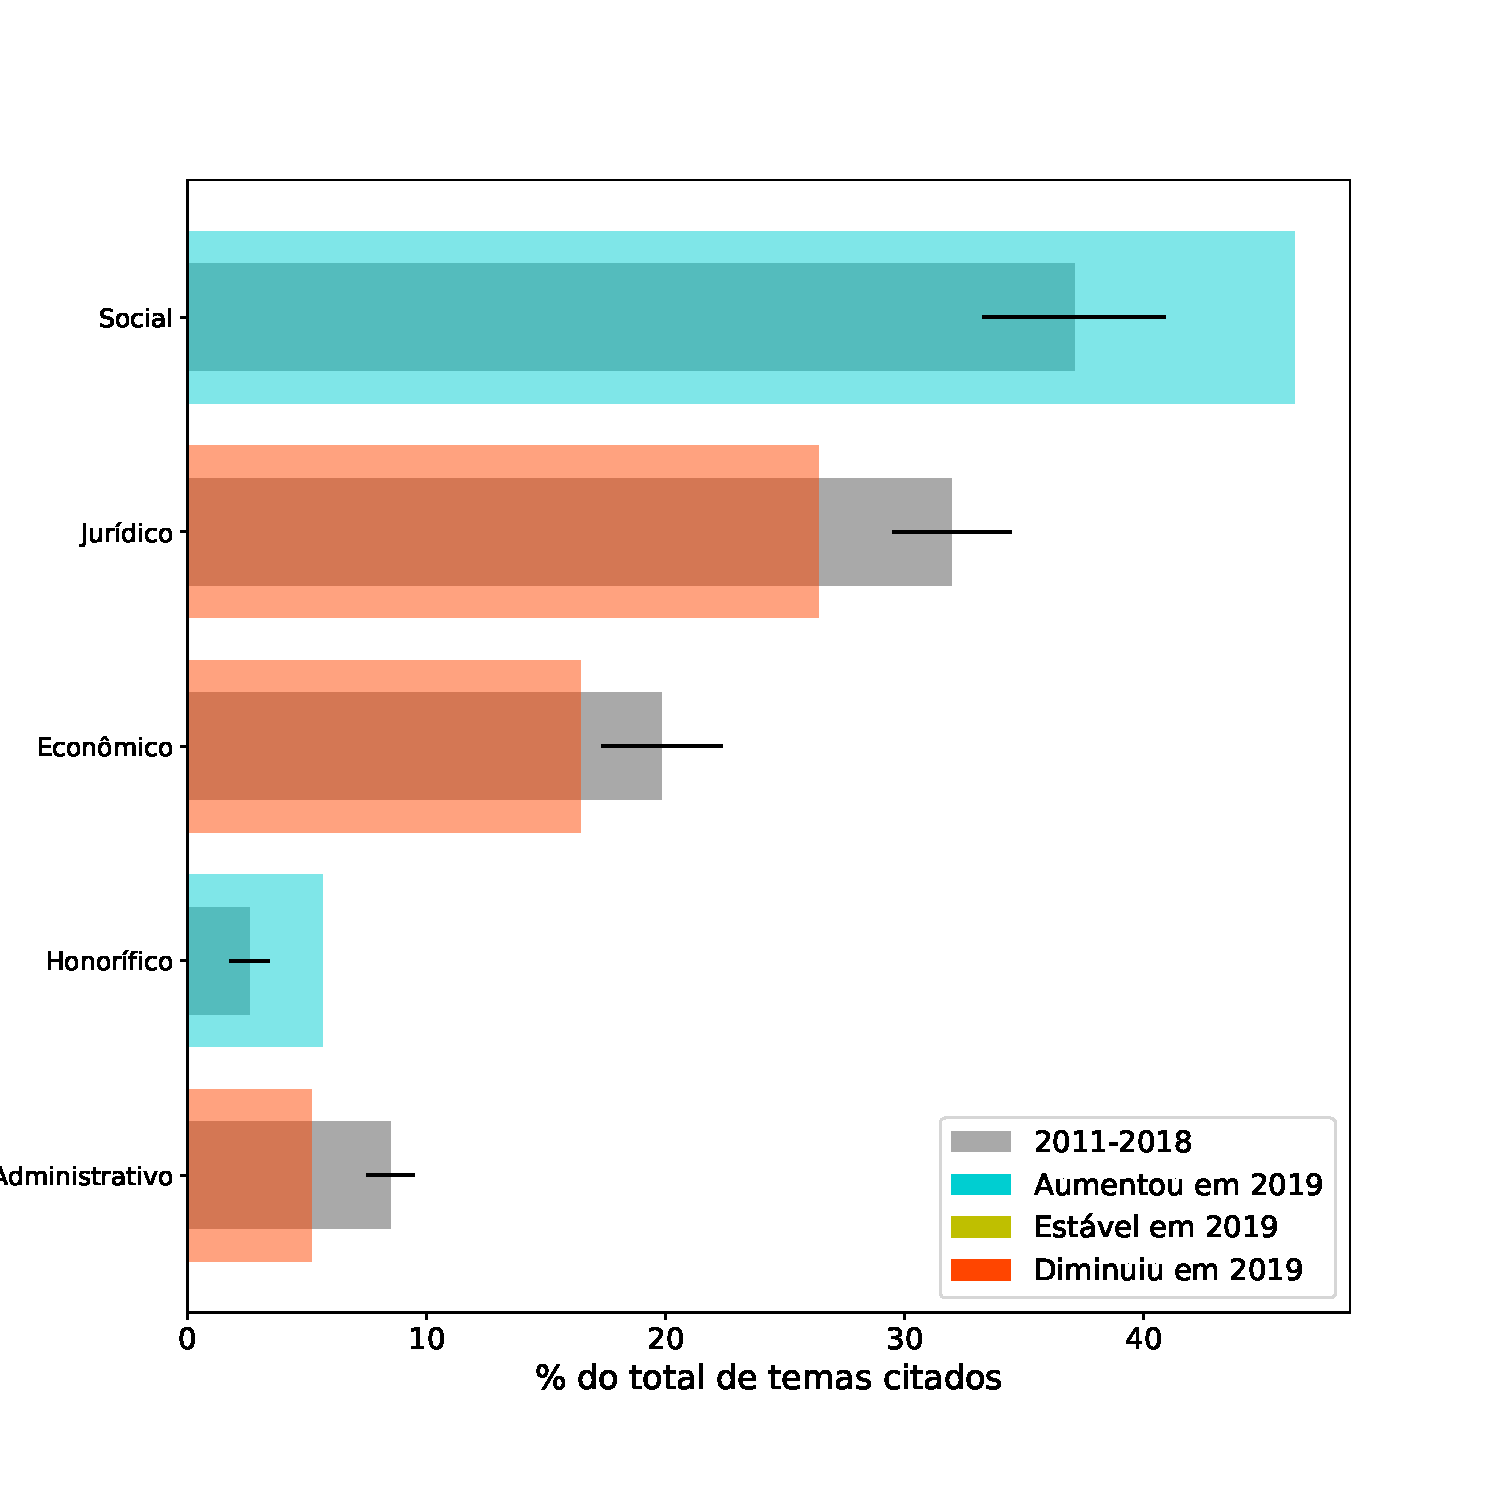
\includegraphics[width=0.7\textwidth]{graficos/senado/pls-macro-temas-senado-r-completo.pdf}
\caption{Frequência de cada macro-tema (fração dos PLs apresentados que foram classificados
  naquele macro-tema) no senado. A representação e a forma de calcular a média histórica são iguais
  aos da Fig. \ref{fig:pl-por-tema-camara}.}
\label{fig:pl-por-macrotema-senado}
\end{figure}

\HX{Incluir tabela com dados sobre temas}

%%%%%%%%%%%%%%%%%%%%%%%%%%%%
\section{Tabelas}
{\footnotesize
\begin{longtable}{llrrr}
  \caption{Lista de deputados da atual legislatura, junto com seu último partido, a fração de votos
  alinhados com o governo, o número de votações com orientações dadas pelo partido no qual o deputado participou,
  e a fração de votos alinhados com o partido. No período em questão, houve 44 votações, sendo que o
  governo orientou o voto em 25 delas.}\\
  \toprule
                                Nome &        Partido &  Al. gov. &  \# Or. part. &  Al. part. \\
                                &                &           &              &            \\
\midrule
\endhead
\midrule
\multicolumn{5}{r}{{Continued on next page}} \\
\midrule
\endfoot
\bottomrule
\endlastfoot
                       André Janones &         Avante &      50,0 &            1 &      100,0 \\
                    Chiquinho Brazão &         Avante &      80,0 &            1 &      100,0 \\
                        Greyce Elias &         Avante &      73,9 &            0 &          - \\
                         Leda Sadala &         Avante &      52,9 &            1 &      100,0 \\
                           Luis Tibé &         Avante &     100,0 &            0 &          - \\
            Pastor Sargento Isidório &         Avante &      21,1 &            1 &        0,0 \\
                                Tito &         Avante &      58,3 &            1 &      100,0 \\
                        Alex Manente &      Cidadania &     100,0 &           38 &       94,7 \\
                      Arnaldo Jardim &      Cidadania &     100,0 &           38 &       97,4 \\
                      Carmen Zanotto &      Cidadania &     100,0 &           38 &       97,4 \\
                          Da Vitória &      Cidadania &      91,7 &           39 &       94,9 \\
                       Daniel Coelho &      Cidadania &     100,0 &           33 &      100,0 \\
                      Marcelo Calero &      Cidadania &      96,0 &           43 &       93,0 \\
                      Paula Belmonte &      Cidadania &     100,0 &           40 &       97,5 \\
                        Rubens Bueno &      Cidadania &     100,0 &           41 &      100,0 \\
                           Alan Rick &            DEM &     100,0 &            1 &      100,0 \\
                     Alexandre Leite &            DEM &     100,0 &            1 &      100,0 \\
                Arthur Oliveira Maia &            DEM &     100,0 &            1 &      100,0 \\
                         Bilac Pinto &            DEM &     100,0 &            0 &          - \\
              Carlos Henrique Gaguim &            DEM &      96,0 &            1 &      100,0 \\
                        David Soares &            DEM &      93,3 &            1 &      100,0 \\
                 Dr. Zacharias Calil &            DEM &     100,0 &            0 &          - \\
                        Efraim Filho &            DEM &     100,0 &            0 &          - \\
                    Eli Corrêa Filho &            DEM &     100,0 &            1 &      100,0 \\
                    Elmar Nascimento &            DEM &     100,0 &            0 &          - \\
               Fernando Coelho Filho &            DEM &     100,0 &            0 &          - \\
                     Geninho Zuliani &            DEM &     100,0 &            0 &          - \\
                         Hélio Leite &            DEM &     100,0 &            1 &      100,0 \\
                Jose Mario Schreiner &            DEM &     100,0 &            1 &      100,0 \\
                     Juninho do Pneu &            DEM &      96,0 &            1 &      100,0 \\
                     Juscelino Filho &            DEM &     100,0 &            1 &      100,0 \\
                       Kim Kataguiri &            DEM &      95,7 &            0 &          - \\
                 Leur Lomanto Júnior &            DEM &     100,0 &            1 &      100,0 \\
                        Luis Miranda &            DEM &     100,0 &            1 &        0,0 \\
                          Norma Ayub &            DEM &     100,0 &            1 &      100,0 \\
                      Olival Marques &            DEM &     100,0 &            1 &      100,0 \\
                           Paulo Azi &            DEM &     100,0 &            1 &      100,0 \\
                        Pedro Lupion &            DEM &      95,5 &            1 &      100,0 \\
                         Pedro Paulo &            DEM &     100,0 &            1 &      100,0 \\
   Professora Dorinha Seabra Rezende &            DEM &      91,7 &            1 &      100,0 \\
                        Rodrigo Maia &            DEM &     100,0 &            0 &          - \\
                 Sóstenes Cavalcante &            DEM &      88,2 &            0 &          - \\
                       Alceu Moreira &            MDB &     100,0 &            1 &      100,0 \\
                        Baleia Rossi &            MDB &      90,9 &            1 &      100,0 \\
                     Carlos Chiodini &            MDB &     100,0 &            1 &        0,0 \\
                      Celso Maldaner &            MDB &     100,0 &            1 &        0,0 \\
                 Daniela do Waguinho &            MDB &      96,0 &            1 &      100,0 \\
                    Darcísio Perondi &            MDB &     100,0 &            1 &      100,0 \\
                       Dulce Miranda &            MDB &      94,4 &            1 &      100,0 \\
                    Elcione Barbalho &            MDB &     100,0 &            0 &          - \\
                          Fabio Reis &            MDB &     100,0 &            1 &      100,0 \\
                       Flaviano Melo &            MDB &      92,3 &            0 &          - \\
                       Fábio Ramalho &            MDB &      91,3 &            1 &      100,0 \\
                      Giovani Feltes &            MDB &     100,0 &            1 &      100,0 \\
                      Gutemberg Reis &            MDB &      95,5 &            1 &      100,0 \\
                    Herculano Passos &            MDB &     100,0 &            1 &      100,0 \\
               Hercílio Coelho Diniz &            MDB &      90,0 &            1 &      100,0 \\
                  Hermes Parcianello &            MDB &      63,6 &            1 &      100,0 \\
                         Hildo Rocha &            MDB &      96,0 &            1 &      100,0 \\
                 Isnaldo Bulhões Jr. &            MDB &     100,0 &            0 &          - \\
                        José Priante &            MDB &     100,0 &            1 &      100,0 \\
                  João Marcelo Souza &            MDB &     100,0 &            1 &      100,0 \\
                        Juarez Costa &            MDB &      87,0 &            1 &      100,0 \\
                       Jéssica Sales &            MDB &      89,5 &            0 &          - \\
                      Lucio Mosquini &            MDB &      76,2 &            1 &      100,0 \\
              Marcos Aurélio Sampaio &            MDB &     100,0 &            1 &      100,0 \\
                         Mauro Lopes &            MDB &     100,0 &            1 &      100,0 \\
                     Moses Rodrigues &            MDB &     100,0 &            0 &          - \\
                      Márcio Biolchi &            MDB &     100,0 &            1 &      100,0 \\
                   Newton Cardoso Jr &            MDB &      75,0 &            1 &      100,0 \\
                          Raul Henry &            MDB &      96,0 &            1 &      100,0 \\
            Rogério Peninha Mendonça &            MDB &      75,0 &            1 &        0,0 \\
                        Sergio Souza &            MDB &     100,0 &            1 &      100,0 \\
                    Valtenir Pereira &            MDB &      92,9 &            0 &          - \\
                      Vinicius Farah &            MDB &      90,9 &            1 &      100,0 \\
                        Walter Alves &            MDB &     100,0 &            1 &      100,0 \\
                     Adriana Ventura &           NOVO &     100,0 &           40 &      100,0 \\
                     Alexis Fonteyne &           NOVO &     100,0 &           41 &      100,0 \\
                      Gilson Marques &           NOVO &     100,0 &           41 &      100,0 \\
                      Lucas Gonzalez &           NOVO &      96,0 &           40 &      100,0 \\
                   Marcel van Hattem &           NOVO &      96,0 &           38 &      100,0 \\
                        Paulo Ganime &           NOVO &      92,3 &           40 &      100,0 \\
                       Tiago Mitraud &           NOVO &      92,0 &           41 &      100,0 \\
                       Vinicius Poit &           NOVO &     100,0 &           41 &       97,6 \\
                      Alice Portugal &          PCdoB &      20,8 &           15 &      100,0 \\
                      Daniel Almeida &          PCdoB &      10,5 &            9 &      100,0 \\
                     Jandira Feghali &          PCdoB &      22,7 &           12 &      100,0 \\
                        Márcio Jerry &          PCdoB &      25,0 &           15 &       93,3 \\
                       Orlando Silva &          PCdoB &      25,0 &           14 &      100,0 \\
                    Perpétua Almeida &          PCdoB &      21,7 &           15 &      100,0 \\
               Professora Marcivania &          PCdoB &       5,6 &           10 &      100,0 \\
                   Renildo Calheiros &          PCdoB &      20,8 &           12 &      100,0 \\
               Rubens Pereira Júnior &          PCdoB &      14,3 &            0 &          - \\
                        Afonso Motta &            PDT &      53,8 &           25 &       96,0 \\
                        Alex Santana &            PDT &      57,1 &           20 &       95,0 \\
                    André Figueiredo &            PDT &      52,4 &           24 &       95,8 \\
                      Chico D`Angelo &            PDT &      26,1 &           21 &       95,2 \\
                  Dagoberto Nogueira &            PDT &      50,0 &           24 &      100,0 \\
                    Damião Feliciano &            PDT &      66,7 &           22 &       90,9 \\
                    Eduardo Bismarck &            PDT &      56,0 &           25 &       92,0 \\
                       Flávia Morais &            PDT &      68,4 &           21 &       95,2 \\
                     Flávio Nogueira &            PDT &      52,0 &           25 &      100,0 \\
                      Fábio Henrique &            PDT &      56,0 &           24 &       95,8 \\
               Félix Mendonça Júnior &            PDT &      61,9 &           22 &       95,5 \\
                          Gil Cutrim &            PDT &      57,7 &           26 &       96,2 \\
                       Gustavo Fruet &            PDT &      60,0 &           23 &      100,0 \\
                     Idilvan Alencar &            PDT &      53,8 &           25 &       92,0 \\
                        Jesus Sérgio &            PDT &      34,8 &           25 &       92,0 \\
                   Leônidas Cristino &            PDT &      41,7 &           25 &       96,0 \\
                       Marlon Santos &            PDT &      40,0 &           18 &      100,0 \\
               Mauro Benevides Filho &            PDT &      50,0 &           19 &       89,5 \\
                      Mário Heringer &            PDT &      64,3 &           11 &       90,9 \\
                         Paulo Ramos &            PDT &      43,5 &           22 &       95,5 \\
                    Pompeo de Mattos &            PDT &      60,9 &           22 &      100,0 \\
                    Robério Monteiro &            PDT &      53,8 &           25 &       96,0 \\
                      Sergio Vidigal &            PDT &      50,0 &           20 &       90,0 \\
                     Silvia Cristina &            PDT &      56,0 &           25 &       96,0 \\
                  Subtenente Gonzaga &            PDT &      66,7 &           20 &       95,0 \\
                       Tabata Amaral &            PDT &      59,1 &           21 &       95,2 \\
                       Túlio Gadêlha &            PDT &      33,3 &           25 &       92,0 \\
                      Wolney Queiroz &            PDT &      31,8 &           21 &      100,0 \\
                       Igor Kannário &            PHS &      95,8 &            4 &      100,0 \\
                         Marcelo Aro &            PHS &     100,0 &            1 &      100,0 \\
                      Eduardo Braide &            PMN &      83,3 &            0 &          - \\
                   Pastor Gildenemyr &            PMN &     100,0 &            0 &          - \\
                            Zé Vitor &            PMN &     100,0 &            2 &      100,0 \\
                     Uldurico Junior &            PPL &      59,1 &            5 &      100,0 \\
                      Abílio Santana &             PR &      83,3 &            2 &      100,0 \\
                      Altineu Côrtes &             PR &     100,0 &            3 &      100,0 \\
                         Bosco Costa &             PR &      96,0 &            4 &      100,0 \\
                     Capitão Augusto &             PR &     100,0 &            3 &       66,7 \\
                 Capitão Fábio Abreu &             PR &     100,0 &            1 &      100,0 \\
           Christiane de Souza Yared &             PR &      94,4 &            4 &      100,0 \\
                      Cristiano Vale &             PR &     100,0 &            4 &      100,0 \\
                          Dr. Jaziel &             PR &     100,0 &            4 &      100,0 \\
                          Edio Lopes &             PR &      94,7 &            1 &      100,0 \\
                    Fernando Rodolfo &             PR &      96,2 &            2 &      100,0 \\
                       Flávia Arruda &             PR &     100,0 &            2 &       50,0 \\
                      Gelson Azevedo &             PR &      96,2 &            1 &      100,0 \\
                             Giacobo &             PR &     100,0 &            0 &          - \\
                     Giovani Cherini &             PR &     100,0 &            4 &      100,0 \\
               Josimar Maranhãozinho &             PR &      96,0 &            1 &      100,0 \\
                          José Rocha &             PR &     100,0 &            2 &      100,0 \\
                 João Carlos Bacelar &             PR &     100,0 &            2 &      100,0 \\
                           João Maia &             PR &     100,0 &            3 &      100,0 \\
                     Junior Lourenço &             PR &     100,0 &            3 &      100,0 \\
                         Júnior Mano &             PR &      92,3 &           14 &       92,9 \\
                            Lauriete &             PR &     100,0 &            4 &      100,0 \\
                     Lincoln Portela &             PR &     100,0 &            3 &      100,0 \\
                   Luiz Carlos Motta &             PR &     100,0 &            3 &       66,7 \\
                      Luiz Nishimori &             PR &     100,0 &            4 &      100,0 \\
                       Magda Mofatto &             PR &      82,4 &            4 &      100,0 \\
                       Marcelo Ramos &             PR &     100,0 &            4 &      100,0 \\
                       Marcio Alvino &             PR &     100,0 &            4 &       75,0 \\
                     Miguel Lombardi &             PR &     100,0 &            4 &      100,0 \\
                        Paulo Freire &             PR &     100,0 &            1 &      100,0 \\
               Policial Katia Sastre &             PR &     100,0 &            3 &      100,0 \\
                      Raimundo Costa &             PR &      96,0 &            2 &      100,0 \\
                  Sebastião Oliveira &             PR &     100,0 &            2 &      100,0 \\
                       Sergio Toledo &             PR &      84,0 &            4 &      100,0 \\
                       Soraya Santos &             PR &     100,0 &            0 &          - \\
                            Tiririca &             PR &      92,3 &            3 &      100,0 \\
                   Vicentinho Júnior &             PR &     100,0 &            4 &      100,0 \\
                  Wellington Roberto &             PR &      66,7 &            2 &      100,0 \\
                        Aline Gurgel &            PRB &      70,6 &           15 &       86,7 \\
                          Amaro Neto &            PRB &      84,6 &           25 &       96,0 \\
                      Aroldo Martins &            PRB &      83,3 &           25 &      100,0 \\
                      Benes Leocádio &            PRB &     100,0 &           25 &       92,0 \\
                Capitão Alberto Neto &            PRB &      96,2 &           23 &       87,0 \\
                        Carlos Gomes &            PRB &      88,5 &           24 &      100,0 \\
                    Celso Russomanno &            PRB &      63,2 &           15 &       86,7 \\
                        Cleber Verde &            PRB &     100,0 &           22 &       86,4 \\
                     Gilberto Abramo &            PRB &      79,2 &           25 &       88,0 \\
                          Hugo Motta &            PRB &      88,2 &           20 &       80,0 \\
                         Hélio Costa &            PRB &      76,0 &           23 &       95,7 \\
                   Jhonatan de Jesus &            PRB &      83,3 &           20 &      100,0 \\
                          Jorge Braz &            PRB &      76,0 &           25 &       96,0 \\
                         João Campos &            PRB &      94,4 &           16 &       87,5 \\
                           João Roma &            PRB &      91,3 &           22 &       90,9 \\
                 Julio Cesar Ribeiro &            PRB &      79,2 &           25 &       92,0 \\
                Lafayette de Andrada &            PRB &      87,5 &           21 &       85,7 \\
                       Manuel Marcos &            PRB &      87,0 &           25 &       96,0 \\
                      Marcos Pereira &            PRB &      84,6 &            9 &      100,0 \\
                         Maria Rosas &            PRB &      79,2 &           24 &       95,8 \\
                       Milton Vieira &            PRB &      79,2 &           23 &       95,7 \\
                      Márcio Marinho &            PRB &      56,5 &           24 &       91,7 \\
                       Ossesio Silva &            PRB &      79,2 &           25 &       96,0 \\
            Professor Luizão Goulart &            PRB &      69,2 &           25 &       88,0 \\
                       Roberto Alves &            PRB &      80,0 &           24 &       95,8 \\
                     Rosangela Gomes &            PRB &      93,3 &           11 &      100,0 \\
                     Severino Pessoa &            PRB &      72,2 &           15 &       93,3 \\
                        Silas Câmara &            PRB &      90,9 &           21 &       85,7 \\
                  Silvio Costa Filho &            PRB &      95,5 &           22 &       90,9 \\
                        Vavá Martins &            PRB &      78,3 &           23 &       91,3 \\
                   Vinicius Carvalho &            PRB &      46,7 &           12 &       83,3 \\
                      Acácio Favacho &           PROS &      91,3 &            8 &       87,5 \\
                         Boca Aberta &           PROS &      80,0 &            1 &      100,0 \\
                      Capitão Wagner &           PROS &      66,7 &            7 &      100,0 \\
                  Clarissa Garotinho &           PROS &      40,0 &            6 &       83,3 \\
                       Eros Biondini &           PROS &     100,0 &            8 &       87,5 \\
                       Gastão Vieira &           PROS &      80,0 &            7 &      100,0 \\
                  Toninho Wandscheer &           PROS &     100,0 &            8 &       87,5 \\
                     Vaidon Oliveira &           PROS &      75,0 &            9 &      100,0 \\
                       Weliton Prado &           PROS &      16,7 &            6 &      100,0 \\
                   Alcides Rodrigues &            PRP &     100,0 &            5 &      100,0 \\
                    Alessandro Molon &            PSB &      29,2 &           31 &      100,0 \\
                       Aliel Machado &            PSB &      41,7 &           30 &      100,0 \\
                     Bira do Pindaré &            PSB &      25,0 &           33 &       93,9 \\
                   Camilo Capiberibe &            PSB &      16,7 &           31 &       93,5 \\
                      Cássio Andrade &            PSB &      44,0 &           32 &      100,0 \\
                       Danilo Cabral &            PSB &      33,3 &           30 &       93,3 \\
                       Denis Bezerra &            PSB &      30,8 &           33 &      100,0 \\
                           Elias Vaz &            PSB &      27,3 &           31 &       90,3 \\
                    Emidinho Madeira &            PSB &      88,0 &           31 &       61,3 \\
                     Felipe Carreras &            PSB &      76,5 &           16 &      100,0 \\
                       Felipe Rigoni &            PSB &      65,2 &           28 &       78,6 \\
                       Gervásio Maia &            PSB &      46,2 &           32 &       96,9 \\
                    Gonzaga Patriota &            PSB &       0,0 &            7 &       85,7 \\
                       Heitor Schuch &            PSB &      26,7 &           20 &       95,0 \\
                    Jefferson Campos &            PSB &      66,7 &           30 &       90,0 \\
                                 Jhc &            PSB &      52,9 &           23 &       95,7 \\
                      João H. Campos &            PSB &      34,6 &           32 &       96,9 \\
                       Júlio Delgado &            PSB &      50,0 &           30 &      100,0 \\
                       Liziane Bayer &            PSB &      77,8 &           19 &      100,0 \\
                       Luciano Ducci &            PSB &      58,3 &           18 &       72,2 \\
                   Luiz Flávio Gomes &            PSB &      25,0 &           28 &       96,4 \\
                      Lídice da Mata &            PSB &      30,0 &           24 &       95,8 \\
                        Marcelo Nilo &            PSB &      34,6 &           31 &      100,0 \\
                         Mauro Nazif &            PSB &      56,5 &           28 &       96,4 \\
                        Rafael Motta &            PSB &      47,4 &           21 &      100,0 \\
                   Rodrigo Agostinho &            PSB &      45,8 &           31 &      100,0 \\
                      Rodrigo Coelho &            PSB &      77,3 &           27 &       74,1 \\
                        Rosana Valle &            PSB &      58,3 &           30 &      100,0 \\
                       Tadeu Alencar &            PSB &      11,8 &           21 &       95,2 \\
                           Ted Conti &            PSB &      30,4 &           32 &      100,0 \\
                   Vilson da Fetaemg &            PSB &      29,2 &           29 &       96,6 \\
                          Átila Lira &            PSB &     100,0 &           28 &       46,4 \\
                      André Ferreira &            PSC &     100,0 &            0 &          - \\
                  Euclydes Pettersen &            PSC &     100,0 &            1 &      100,0 \\
                 Gilberto Nascimento &            PSC &     100,0 &            1 &        0,0 \\
                      Glaustin Fokus &            PSC &     100,0 &            0 &          - \\
                       Osires Damaso &            PSC &      88,0 &            1 &        0,0 \\
                      Otoni de Paula &            PSC &     100,0 &            1 &      100,0 \\
               Paulo Eduardo Martins &            PSC &     100,0 &            1 &      100,0 \\
                    Valdevan Noventa &            PSC &      75,0 &            0 &          - \\
                 Alexandre Serfiotis &            PSD &      90,5 &           34 &       88,2 \\
                      André de Paula &            PSD &     100,0 &           32 &       93,8 \\
                       Antonio Brito &            PSD &      92,3 &           21 &       90,5 \\
                Cezinha de Madureira &            PSD &     100,0 &           28 &       92,9 \\
                   Charles Fernandes &            PSD &      76,9 &           39 &       71,8 \\
          Danrlei de Deus Hinterholz &            PSD &      81,0 &           31 &       71,0 \\
                      Darci de Matos &            PSD &     100,0 &           35 &       91,4 \\
                 Delegado Éder Mauro &            PSD &     100,0 &           30 &      100,0 \\
                       Diego Andrade &            PSD &     100,0 &           27 &       92,6 \\
                       Domingos Neto &            PSD &      95,2 &           29 &       96,6 \\
                     Edilázio Júnior &            PSD &     100,0 &           38 &       94,7 \\
                       Evandro Roman &            PSD &     100,0 &           20 &      100,0 \\
                      Expedito Netto &            PSD &      31,6 &           29 &       34,5 \\
                           Flordelis &            PSD &     100,0 &           25 &       92,0 \\
                       Francisco Jr. &            PSD &     100,0 &           34 &       94,1 \\
                         Fábio Faria &            PSD &     100,0 &           16 &      100,0 \\
                     Fábio Mitidieri &            PSD &     100,0 &           15 &      100,0 \\
                          Fábio Trad &            PSD &      88,0 &           38 &       89,5 \\
                   Haroldo Cathedral &            PSD &      90,9 &           32 &       90,6 \\
                           Hugo Leal &            PSD &     100,0 &           30 &       96,7 \\
                  Joaquim Passarinho &            PSD &     100,0 &           37 &       91,9 \\
                          José Nunes &            PSD &     100,0 &           34 &       97,1 \\
                         Júlio Cesar &            PSD &     100,0 &           30 &       96,7 \\
                      Júnior Ferrari &            PSD &     100,0 &           39 &       92,3 \\
                    Marco Bertaiolli &            PSD &     100,0 &           37 &       97,3 \\
                        Marx Beltrão &            PSD &      95,5 &           33 &       93,9 \\
                      Misael Varella &            PSD &      90,9 &           13 &       92,3 \\
                  Otto Alencar Filho &            PSD &      70,8 &           36 &       66,7 \\
                     Paulo Magalhães &            PSD &      92,9 &           18 &       94,4 \\
           Reinhold Stephanes Junior &            PSD &     100,0 &           26 &       96,2 \\
                       Ricardo Guidi &            PSD &     100,0 &           35 &       94,3 \\
                      Sargento Fahur &            PSD &     100,0 &           39 &       94,9 \\
                        Sidney Leite &            PSD &     100,0 &           35 &       94,3 \\
                      Stefano Aguiar &            PSD &     100,0 &           21 &      100,0 \\
                        Sérgio Brito &            PSD &     100,0 &           10 &      100,0 \\
                            Vermelho &            PSD &     100,0 &           31 &      100,0 \\
                  Wladimir Garotinho &            PSD &      75,0 &           18 &       88,9 \\
                        Adolfo Viana &           PSDB &     100,0 &            8 &      100,0 \\
                         Aécio Neves &           PSDB &     100,0 &            7 &      100,0 \\
                        Beto Pereira &           PSDB &      96,0 &            7 &      100,0 \\
                         Bia Cavassa &           PSDB &     100,0 &            8 &      100,0 \\
                        Bruna Furlan &           PSDB &      92,9 &            5 &      100,0 \\
                      Carlos Sampaio &           PSDB &      80,0 &            3 &      100,0 \\
                        Celso Sabino &           PSDB &      88,0 &            8 &      100,0 \\
                      Célio Silveira &           PSDB &      91,3 &            6 &      100,0 \\
                     Daniel Trzeciak &           PSDB &     100,0 &            8 &      100,0 \\
                      Domingos Sávio &           PSDB &     100,0 &            7 &      100,0 \\
                       Edna Henrique &           PSDB &      88,9 &            1 &      100,0 \\
                     Eduardo Barbosa &           PSDB &      84,0 &            7 &       85,7 \\
                        Eduardo Cury &           PSDB &     100,0 &            8 &       87,5 \\
                      Geovania de Sá &           PSDB &      94,7 &            4 &      100,0 \\
                      Lucas Redecker &           PSDB &     100,0 &            7 &      100,0 \\
                         Luiz Carlos &           PSDB &     100,0 &            7 &      100,0 \\
                          Mara Rocha &           PSDB &     100,0 &            8 &      100,0 \\
                    Mariana Carvalho &           PSDB &     100,0 &            5 &       80,0 \\
                        Nilson Pinto &           PSDB &     100,0 &            8 &      100,0 \\
                     Paulo Abi-Ackel &           PSDB &     100,0 &            6 &      100,0 \\
                    Pedro Cunha Lima &           PSDB &      95,8 &            7 &       71,4 \\
                      Roberto Pessoa &           PSDB &     100,0 &            1 &      100,0 \\
                   Rodrigo de Castro &           PSDB &     100,0 &            8 &       87,5 \\
                        Rose Modesto &           PSDB &      95,8 &            7 &      100,0 \\
                        Ruy Carneiro &           PSDB &      91,3 &            7 &      100,0 \\
                      Samuel Moreira &           PSDB &      96,0 &            8 &       87,5 \\
                            Shéridan &           PSDB &      94,4 &            8 &       87,5 \\
                        Tereza Nelma &           PSDB &      81,0 &            7 &      100,0 \\
                    Vanderlei Macris &           PSDB &     100,0 &            8 &      100,0 \\
                         Vitor Lippi &           PSDB &      95,2 &            7 &       85,7 \\
                           Abou Anni &            PSL &     100,0 &           35 &       94,3 \\
                     Alexandre Frota &            PSL &     100,0 &           39 &       92,3 \\
                      Aline Sleutjes &            PSL &     100,0 &           22 &       86,4 \\
                           Alê Silva &            PSL &     100,0 &           37 &       91,9 \\
                           Bia Kicis &            PSL &      95,2 &           32 &       90,6 \\
                          Bibo Nunes &            PSL &     100,0 &           35 &       91,4 \\
                   Cabo Junio Amaral &            PSL &     100,0 &           35 &       94,3 \\
                      Carla Zambelli &            PSL &     100,0 &           34 &       94,1 \\
                        Carlos Jordy &            PSL &     100,0 &           37 &       91,9 \\
                    Caroline de Toni &            PSL &     100,0 &           37 &       86,5 \\
                Charlles Evangelista &            PSL &     100,0 &           35 &       94,3 \\
                      Chris Tonietto &            PSL &     100,0 &           35 &       94,3 \\
                     Coronel Armando &            PSL &     100,0 &           36 &       94,4 \\
                 Coronel Chrisóstomo &            PSL &     100,0 &           34 &       97,1 \\
                       Coronel Tadeu &            PSL &     100,0 &           37 &       89,2 \\
                      Daniel Freitas &            PSL &     100,0 &           39 &       87,2 \\
                     Daniel Silveira &            PSL &     100,0 &           39 &       87,2 \\
            Delegado Antônio Furtado &            PSL &     100,0 &           37 &       97,3 \\
            Delegado Marcelo Freitas &            PSL &     100,0 &           38 &       89,5 \\
                      Delegado Pablo &            PSL &     100,0 &           34 &       97,1 \\
                     Delegado Waldir &            PSL &     100,0 &           22 &      100,0 \\
                     Dr. Luiz Ovando &            PSL &      96,0 &           36 &       94,4 \\
                  Dra. Soraya Manato &            PSL &     100,0 &           39 &       92,3 \\
                   Eduardo Bolsonaro &            PSL &     100,0 &           27 &       96,3 \\
                         Enéias Reis &            PSL &     100,0 &           31 &       96,8 \\
                     Fabio Schiochet &            PSL &     100,0 &           29 &      100,0 \\
                 Felipe Francischini &            PSL &     100,0 &           30 &      100,0 \\
                     Felício Laterça &            PSL &     100,0 &           30 &       90,0 \\
                       Filipe Barros &            PSL &     100,0 &           34 &       97,1 \\
                       General Girão &            PSL &     100,0 &           37 &       94,6 \\
                  General Peternelli &            PSL &     100,0 &           38 &       92,1 \\
                       Guiga Peixoto &            PSL &     100,0 &           39 &       92,3 \\
                              Gurgel &            PSL &     100,0 &           36 &       94,4 \\
                       Heitor Freire &            PSL &     100,0 &           28 &       89,3 \\
                         Helio Lopes &            PSL &     100,0 &           34 &       94,1 \\
                    Joice Hasselmann &            PSL &      93,8 &           25 &       92,0 \\
                        Julian Lemos &            PSL &      96,0 &           34 &       94,1 \\
                     Júnior Bozzella &            PSL &     100,0 &           35 &       97,1 \\
                      Loester Trutis &            PSL &     100,0 &           34 &       97,1 \\
                      Lourival Gomes &            PSL &     100,0 &           37 &       97,3 \\
                       Luciano Bivar &            PSL &     100,0 &            5 &      100,0 \\
                           Luiz Lima &            PSL &     100,0 &           38 &       89,5 \\
 Luiz Philippe de Orleans e Bragança &            PSL &      95,5 &           35 &       88,6 \\
                           Léo Motta &            PSL &     100,0 &           37 &       91,9 \\
                       Major Fabiana &            PSL &     100,0 &           34 &       94,1 \\
                    Major Vitor Hugo &            PSL &     100,0 &           17 &      100,0 \\
                        Marcelo Brum &            PSL &     100,0 &           27 &       96,3 \\
                        Márcio Labre &            PSL &      96,0 &           35 &       94,3 \\
                      Nelson Barbudo &            PSL &     100,0 &           34 &       91,2 \\
                       Nereu Crispim &            PSL &     100,0 &           34 &       97,1 \\
                           Nicoletti &            PSL &     100,0 &           38 &       92,1 \\
                    Professor Joziel &            PSL &     100,0 &           34 &       94,1 \\
          Professora Dayane Pimentel &            PSL &     100,0 &           36 &       94,4 \\
                           Sanderson &            PSL &     100,0 &           29 &       93,1 \\
                       David Miranda &           PSOL &       5,9 &           29 &       89,7 \\
                  Edmilson Rodrigues &           PSOL &      20,0 &           44 &       90,9 \\
                 Fernanda Melchionna &           PSOL &      20,0 &           42 &       92,9 \\
                       Glauber Braga &           PSOL &      20,0 &           43 &       93,0 \\
                        Ivan Valente &           PSOL &      20,0 &           44 &       95,5 \\
                      Luiza Erundina &           PSOL &      80,0 &           10 &       90,0 \\
                      Marcelo Freixo &           PSOL &      21,7 &           41 &       95,1 \\
                        Sâmia Bomfim &           PSOL &      16,7 &           42 &       95,2 \\
                     Talíria Petrone &           PSOL &      16,7 &           43 &       95,3 \\
                      Áurea Carolina &           PSOL &      20,8 &           43 &       95,3 \\
                     Afonso Florence &             PT &      21,7 &           36 &       94,4 \\
                      Airton Faleiro &             PT &      22,7 &           33 &       97,0 \\
               Alencar Santana Braga &             PT &      33,3 &           27 &      100,0 \\
                   Alexandre Padilha &             PT &      38,5 &           26 &      100,0 \\
                   Arlindo Chinaglia &             PT &      29,4 &           31 &      100,0 \\
                      Assis Carvalho &             PT &      28,6 &           23 &      100,0 \\
                   Benedita da Silva &             PT &      29,4 &           24 &      100,0 \\
                           Beto Faro &             PT &      21,7 &           38 &       94,7 \\
                           Bohn Gass &             PT &      22,2 &           31 &       93,5 \\
                        Carlos Veras &             PT &      21,7 &           37 &       91,9 \\
                    Carlos Zarattini &             PT &      20,8 &           38 &       92,1 \\
                         Célio Moura &             PT &      38,9 &           27 &       81,5 \\
                          Enio Verri &             PT &      23,8 &           36 &       97,2 \\
                         Erika Kokay &             PT &      25,0 &           34 &       94,1 \\
              Frei Anastacio Ribeiro &             PT &      22,7 &           36 &       94,4 \\
                     Gleisi Hoffmann &             PT &       0,0 &            7 &       85,7 \\
                      Helder Salomão &             PT &      21,7 &           37 &       97,3 \\
                    Henrique Fontana &             PT &      20,0 &           38 &       84,2 \\
                         Jorge Solla &             PT &      21,1 &           32 &       96,9 \\
                      Joseildo Ramos &             PT &      41,7 &           17 &      100,0 \\
                  José Airton Cirilo &             PT &      46,2 &           20 &       85,0 \\
                      José Guimarães &             PT &      21,7 &           38 &       97,4 \\
                        José Ricardo &             PT &      19,2 &           42 &       92,9 \\
                         João Daniel &             PT &      26,1 &           33 &       90,9 \\
                   Leonardo Monteiro &             PT &      25,0 &           35 &       94,3 \\
                      Luizianne Lins &             PT &       0,0 &           17 &       88,2 \\
                              Marcon &             PT &      33,3 &           35 &       85,7 \\
                   Margarida Salomão &             PT &      25,0 &           33 &       97,0 \\
                    Maria do Rosário &             PT &      30,8 &           25 &       96,0 \\
                      Marília Arraes &             PT &      15,8 &           30 &       96,7 \\
                   Natália Bonavides &             PT &      21,7 &           38 &       94,7 \\
                   Nelson Pellegrino &             PT &      29,4 &           30 &      100,0 \\
                         Nilto Tatto &             PT &      22,7 &           37 &       97,3 \\
                         Odair Cunha &             PT &       8,3 &           21 &       90,5 \\
                          Padre João &             PT &      20,8 &           39 &       97,4 \\
                      Patrus Ananias &             PT &      20,0 &           39 &       89,7 \\
                        Paulo Guedes &             PT &      16,7 &           42 &       90,5 \\
                       Paulo Pimenta &             PT &      12,5 &           13 &      100,0 \\
                      Paulo Teixeira &             PT &       0,0 &           27 &       92,6 \\
                              Paulão &             PT &      22,7 &           35 &       88,6 \\
                         Pedro Uczai &             PT &      22,7 &           38 &       94,7 \\
               Professora Rosa Neide &             PT &      20,8 &           36 &       97,2 \\
                     Reginaldo Lopes &             PT &      23,8 &           35 &      100,0 \\
                         Rejane Dias &             PT &      23,5 &           28 &       96,4 \\
                     Rogério Correia &             PT &      23,8 &           35 &       97,1 \\
                        Rubens Otoni &             PT &       5,0 &           34 &       97,1 \\
                          Rui Falcão &             PT &      26,1 &           38 &       89,5 \\
                     Valmir Assunção &             PT &      20,0 &           40 &       95,0 \\
                       Vander Loubet &             PT &      31,2 &           29 &       96,6 \\
                          Vicentinho &             PT &      22,7 &           36 &       94,4 \\
                    Waldenor Pereira &             PT &      25,0 &           31 &       90,3 \\
                         Zeca Dirceu &             PT &       8,3 &           21 &      100,0 \\
                           Zé Carlos &             PT &      20,8 &           36 &       88,9 \\
                             Zé Neto &             PT &      14,3 &           31 &       96,8 \\
                       Eduardo Costa &            PTB &      80,0 &            1 &      100,0 \\
               Emanuel Pinheiro Neto &            PTB &      90,9 &            0 &          - \\
                      Luisa Canziani &            PTB &      90,5 &            0 &          - \\
                      Marcelo Moraes &            PTB &      64,7 &            1 &      100,0 \\
                 Maurício Dziedricki &            PTB &     100,0 &            1 &      100,0 \\
                 Nivaldo Albuquerque &            PTB &      88,5 &            1 &      100,0 \\
                      Paulo Bengtson &            PTB &      87,5 &            0 &          - \\
               Pedro Augusto Bezerra &            PTB &      82,6 &            1 &      100,0 \\
               Pedro Lucas Fernandes &            PTB &      95,7 &            0 &          - \\
                             Santini &            PTB &      92,0 &            1 &      100,0 \\
                     Wilson Santiago &            PTB &      95,2 &            1 &      100,0 \\
                       Célio Studart &             PV &      60,0 &            1 &      100,0 \\
                       Enrico Misasi &             PV &     100,0 &            1 &      100,0 \\
                             Leandre &             PV &      66,7 &            1 &      100,0 \\
            Professor Israel Batista &             PV &      66,7 &            1 &        0,0 \\
                       Dr. Frederico &       Patriota &      91,7 &           27 &       92,6 \\
                          Fred Costa &       Patriota &     100,0 &           27 &       96,3 \\
                       Marreca Filho &       Patriota &     100,0 &           26 &      100,0 \\
                       Pastor Eurico &       Patriota &     100,0 &           28 &       96,4 \\
                      Aluisio Mendes &        Podemos &      95,0 &           23 &       65,2 \\
                             Bacelar &        Podemos &      12,0 &           23 &       60,9 \\
                        Diego Garcia &        Podemos &      35,0 &           20 &       85,0 \\
                           Igor Timo &        Podemos &      60,0 &           17 &       76,5 \\
                       José Medeiros &        Podemos &      95,0 &           21 &       61,9 \\
                          José Nelto &        Podemos &      62,5 &           15 &       73,3 \\
                          Léo Moraes &        Podemos &      90,5 &           25 &       72,0 \\
                 Pr. Marco Feliciano &        Podemos &      82,6 &           20 &       75,0 \\
                        Renata Abreu &        Podemos &     100,0 &           21 &       57,1 \\
                    Ricardo Teobaldo &        Podemos &      94,7 &           17 &       58,8 \\
                   Roberto de Lucena &        Podemos &      77,3 &           22 &       86,4 \\
                    Adriano do Baldy &  Progressistas &     100,0 &           37 &       94,6 \\
                         Afonso Hamm &  Progressistas &     100,0 &           35 &       97,1 \\
                   Aguinaldo Ribeiro &  Progressistas &      94,1 &           27 &       92,6 \\
                      Aj Albuquerque &  Progressistas &      95,8 &           36 &       94,4 \\
                         André Abdon &  Progressistas &     100,0 &           31 &      100,0 \\
                        André Fufuca &  Progressistas &      60,0 &            6 &       66,7 \\
                         Angela Amin &  Progressistas &     100,0 &           33 &       93,9 \\
                         Arthur Lira &  Progressistas &     100,0 &           12 &      100,0 \\
                         Beto Rosado &  Progressistas &     100,0 &           13 &       76,9 \\
                           Cacá Leão &  Progressistas &     100,0 &           38 &       94,7 \\
                         Celina Leão &  Progressistas &     100,0 &           35 &       97,1 \\
                     Christino Aureo &  Progressistas &     100,0 &           37 &       91,9 \\
                      Claudio Cajado &  Progressistas &     100,0 &           19 &       94,7 \\
                       Dimas Fabiano &  Progressistas &     100,0 &           33 &       93,9 \\
       Dr. Luiz Antonio Teixeira Jr. &  Progressistas &     100,0 &           36 &       94,4 \\
                    Eduardo da Fonte &  Progressistas &     100,0 &           18 &      100,0 \\
                Evair Vieira de Melo &  Progressistas &     100,0 &           21 &       90,5 \\
                       Fausto Pinato &  Progressistas &     100,0 &           16 &       93,8 \\
                   Fernando Monteiro &  Progressistas &      94,4 &           24 &       91,7 \\
                    Franco Cartafina &  Progressistas &     100,0 &           21 &       95,2 \\
                   Guilherme Derrite &  Progressistas &     100,0 &           37 &       89,2 \\
                     Guilherme Mussi &  Progressistas &     100,0 &           20 &       95,0 \\
                     Hiran Gonçalves &  Progressistas &      72,2 &           26 &       73,1 \\
                    Iracema Portella &  Progressistas &     100,0 &           25 &      100,0 \\
                    Jaqueline Cassol &  Progressistas &     100,0 &           35 &       97,1 \\
                    Jerônimo Goergen &  Progressistas &      90,9 &           34 &       88,2 \\
                    Laercio Oliveira &  Progressistas &      95,2 &           32 &       87,5 \\
                    Margarete Coelho &  Progressistas &     100,0 &           36 &       97,2 \\
                Mário Negromonte Jr. &  Progressistas &      92,0 &           38 &       89,5 \\
                         Neri Geller &  Progressistas &      91,7 &           33 &       90,9 \\
                    Pedro Westphalen &  Progressistas &     100,0 &           29 &       96,6 \\
                         Pinheirinho &  Progressistas &     100,0 &           37 &       94,6 \\
                   Professor Alcides &  Progressistas &     100,0 &           38 &       94,7 \\
                      Ricardo Barros &  Progressistas &      83,3 &           18 &       83,3 \\
                        Ricardo Izar &  Progressistas &     100,0 &           32 &       93,8 \\
                    Ronaldo Carletto &  Progressistas &     100,0 &           24 &       91,7 \\
                         Schiavinato &  Progressistas &     100,0 &           39 &       94,9 \\
                          Átila Lins &  Progressistas &     100,0 &           16 &      100,0 \\
                    Joenia Wapichana &           REDE &      75,0 &            7 &      100,0 \\
                 Luiz Antônio Corrêa &        S.Part. &      88,0 &            0 &          - \\
                    Augusto Coutinho &  Solidariedade &      95,2 &           21 &       71,4 \\
                       Aureo Ribeiro &  Solidariedade &      89,5 &           21 &       76,2 \\
                       Bosco Saraiva &  Solidariedade &      95,8 &           27 &       74,1 \\
                        Dr. Leonardo &  Solidariedade &      80,0 &           29 &       79,3 \\
                   Dra. Vanda Milani &  Solidariedade &      70,0 &           24 &       91,7 \\
                          Eli Borges &  Solidariedade &      76,0 &           27 &       88,9 \\
                    Genecias Noronha &  Solidariedade &      73,9 &           25 &       88,0 \\
                    Gustinho Ribeiro &  Solidariedade &      88,0 &           29 &       82,8 \\
                      Lucas Vergilio &  Solidariedade &     100,0 &           15 &       66,7 \\
                       Marina Santos &  Solidariedade &      83,3 &           18 &       88,9 \\
                    Otaci Nascimento &  Solidariedade &      88,0 &           28 &       82,1 \\
              Paulo Pereira da Silva &  Solidariedade &      78,9 &           23 &       87,0 \\
                    Simplício Araújo &  Solidariedade &     100,0 &            0 &          - \\
                         Tiago Dimas &  Solidariedade &      75,0 &           28 &       89,3 \\
                            Zé Silva &  Solidariedade &      73,7 &           25 &       92,0 \\
\label{tab:alinha-dep}
\end{longtable}

}


%%%%%%%%%%%%%%%%%%%%%%%%%%%
\section{Figuras adicionais}

\begin{figure}[H]
\centering
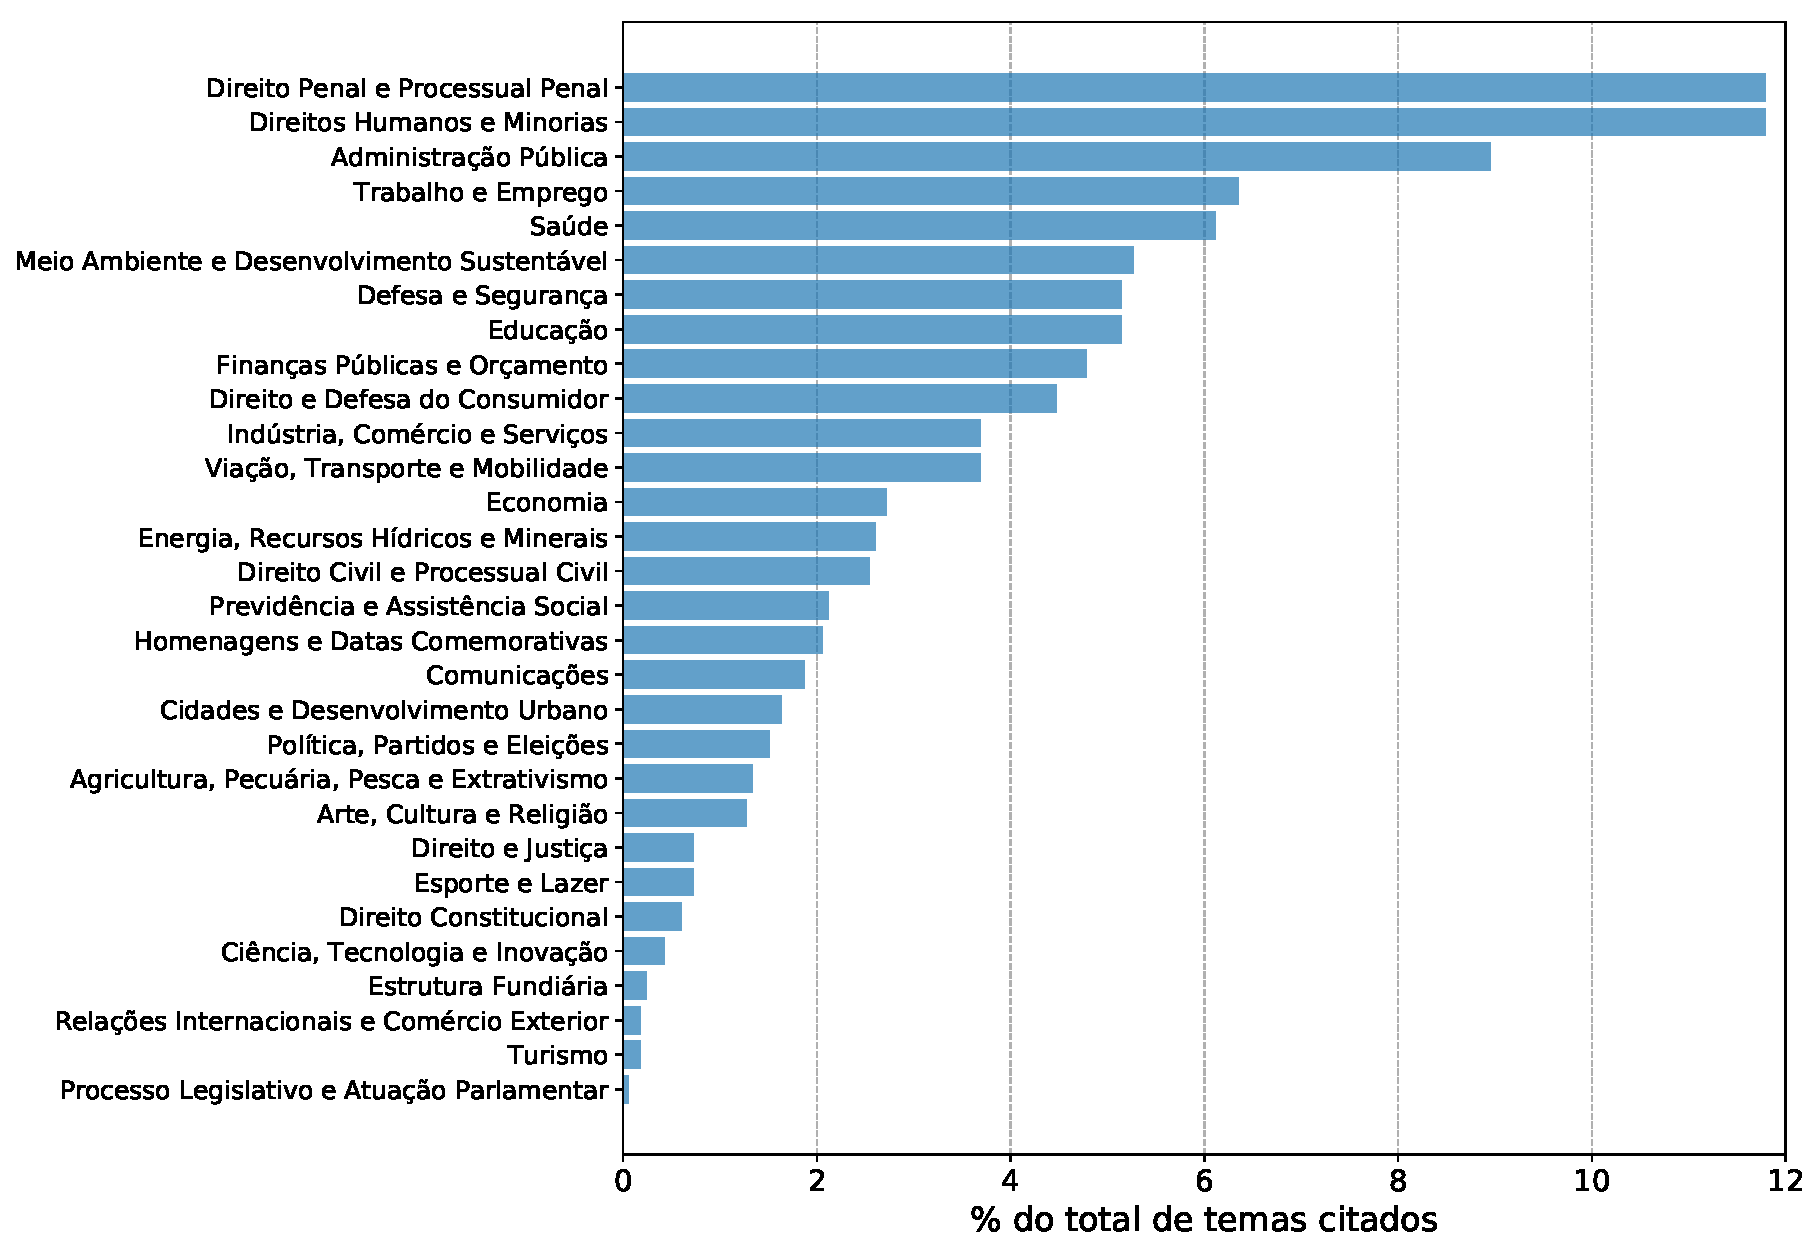
\includegraphics[width=1.0\textwidth]{graficos/temas_PL_fracao2019_2019-05-03.pdf}
\caption{Versão simplificada da Fig. \ref{fig:pl-por-tema-camara}. Aqui apenas apresentamos a frequência com
  que os temas apareceram na câmara nos 100 primeiros dias de 2019, sem comparar com o histórico.}
\label{fig:pl-por-tema-camara-simples}
\end{figure}

\begin{figure}[H]
\centering
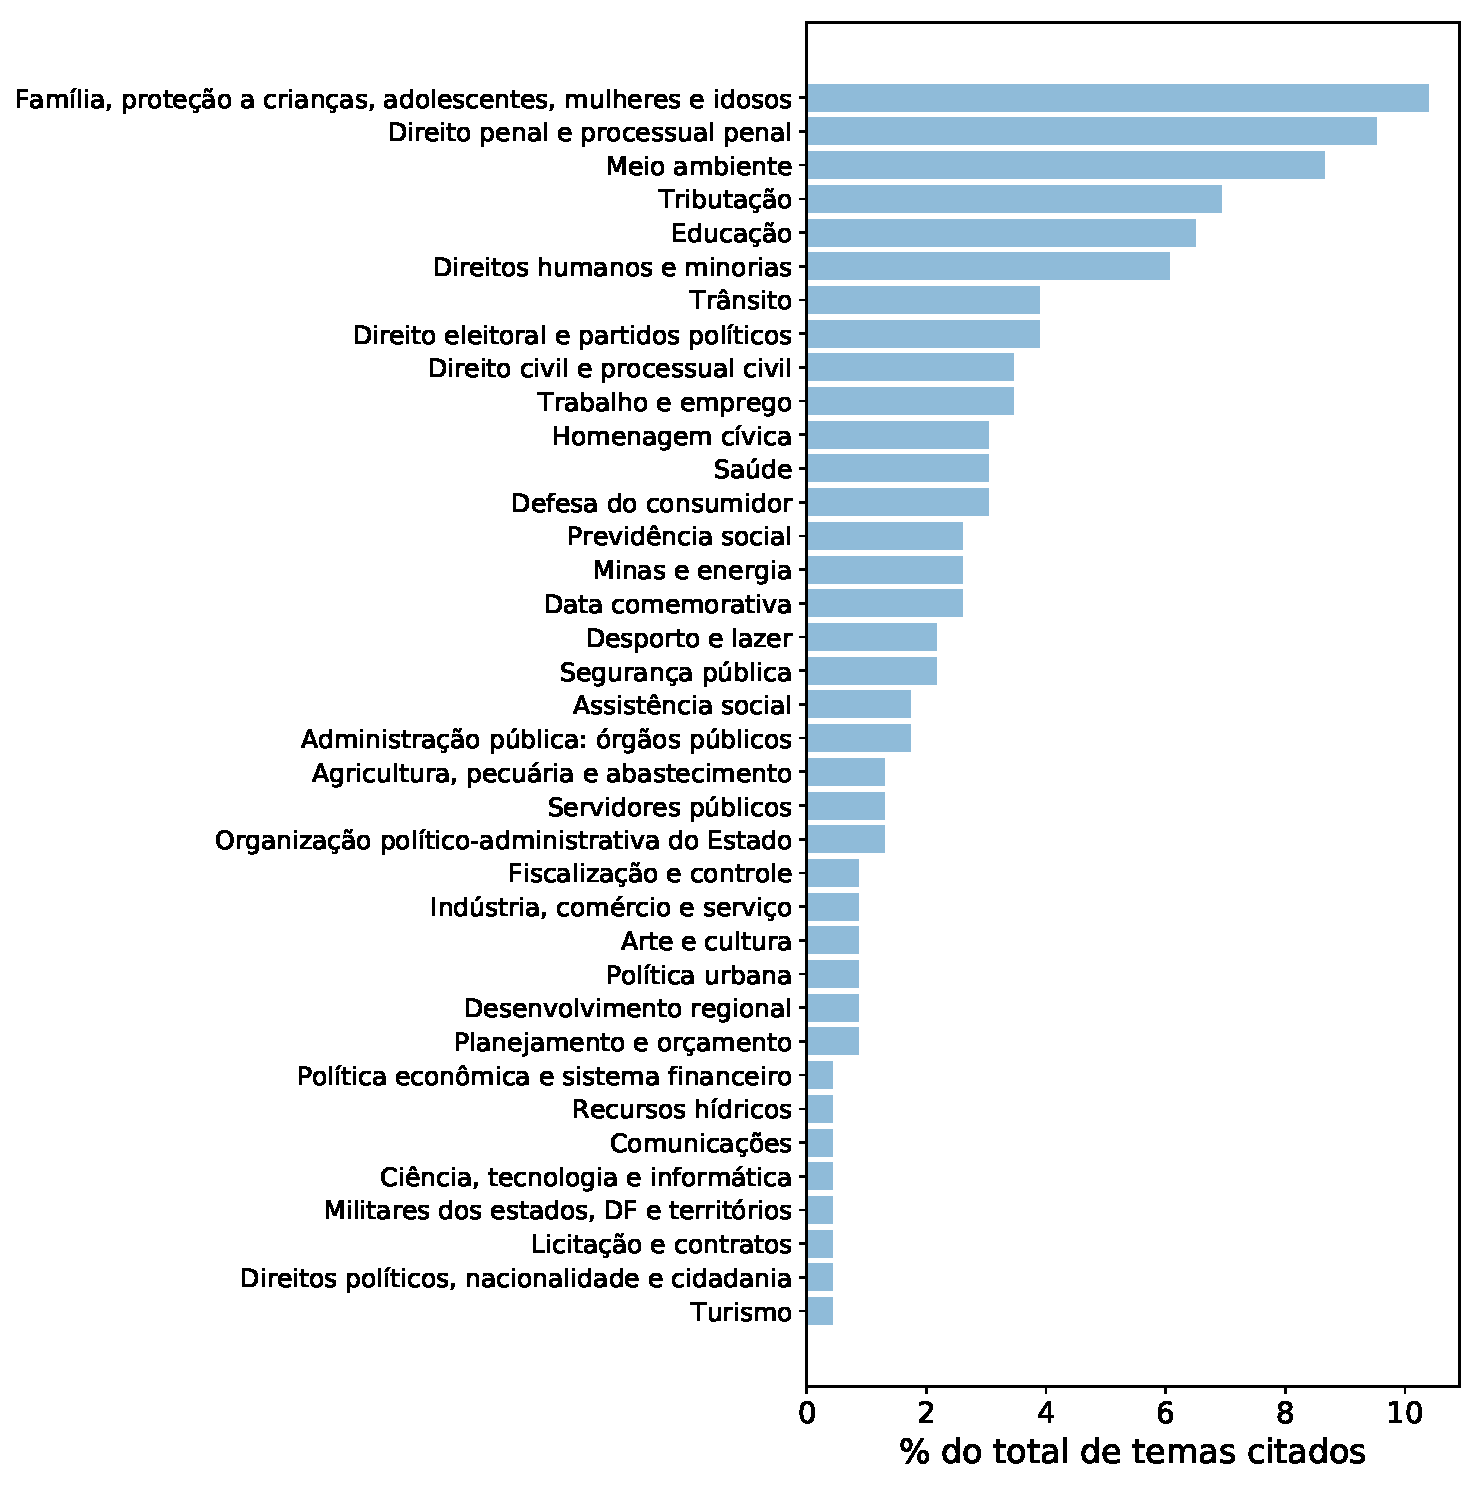
\includegraphics[width=1.0\textwidth]{graficos/senado/pls-temas-senado-r-simples.pdf}
\caption{Versão simplificada da Fig. \ref{fig:pl-por-tema-senado}. Aqui apenas apresentamos a frequência com
  que os temas apareceram no senado nos 100 primeiros dias de 2019, sem comparar com o histórico.}
\label{fig:pl-por-tema-senado-simples}
\end{figure}


\end{document}
